% ===================================================================
% THESIS OVERVIEW
% ===================================================================
\section{Introduction}\label{sec:introduction}

Deep learning has achieved significant performance gains over traditional
methods on various tasks like image
classification~\cite{deng2009imagenet,krizhevsky2012imagenet,zeiler2012visualizing,simonyan2015deep,szegedy2015going,he2016deep},
image
generation~\cite{goodfellow2014generative,choi2020starganv2,karras2018progressive,ramesh2021zero},
machine translation~\cite{bahdanau2014neural,luong2015effective,wu2016google},
and game play~\cite{mnih2013playing,silver2016mastering,silver2018general}.
These applications are powered by machine learning (ML)
frameworks~\cite{tokui2015chainer,chen2015mxnet,paszke2019pytorch,abadi2016tensorflow,}
that tremendously reduce the added complexity for practitioners of using
highly-efficient implementations on hardware accelerators like
GPUs~\cite{kirk2007nvidia} and TPUs~\cite{jouppi2017in}. The convenience
introduced by these libraries makes deep learning more accessible and is one
main factor for its popularity and success.

It is surprisingly easy to build, train, and deploy a model, despite deep
learning being computationally extremely demanding. Typically, neural networks
have
millions~\cite{krizhevsky2012imagenet,zeiler2012visualizing,simonyan2015deep,szegedy2015going,he2016deep},
billions~\cite{radford2019language,brown2020language}, even
trillions~\cite{fedus2022switch} of parameters, and are trained on large data
sets~\cite{deng2009imagenet,lin2014microsoft} that can only be processed in
smaller batches. The parameters are adjusted during training, which is phrased
as optimization of a performance measure called ``the loss''.

Training, \ie optimization, proceeds in an iterative fashion: to update the
model, a mini-batch of data is fed through the model (forward pass) to evaluate
its current performance---the mini-batch loss. This loss is then differentiated
\wrt the model's parameters to obtain the mini-batch gradient (backward pass).
Finally, an optimizer incorporates this gradient to update the model parameters.
Popular frameworks like \pytorch \cite{paszke2019pytorch} and \tensorflow
\cite{abadi2016tensorflow} realize this procedure in code that looks similar to
the following pseudocode:

\begin{lstlisting}[ language=Python, caption={\textbf{Canonical deep learning
training loop.} After setting up the data, model, loss function, and optimizer,
iterate over batches: in each iteration, compute the mini-batch loss in a forward
pass, and its gradient with a backward pass. Then use the gradient as learning
signal to update the model parameters.}, label=alg:background::trainingLoop,
captionpos=t,
linebackgroundcolor={\ifnum\value{lstnumber}=15\color{secondcolor!50}\fi\ifnum\value{lstnumber}=16\color{secondcolor!50}\fi}]
 dataset = ...    # Learning task examples (@\label{line:background::dataset}@)

 model = ...      # Practitioner's choice (@\label{line:background::model}@)
 loss_func = ...  # Practitioner's choice (@\label{line:background::lossFunc}@)

 optimizer = ...  # First-order method

 while not_converged: # Standard training loop
     features, targets = dataset.next_minibatch()

     # Forward pass: Compute the loss
     predictions = model(features)
     loss = loss_func(predictions, targets)

     # Backward pass: Compute the gradient
     loss.backward() (@\label{line:background::Backward}@)

     # Update model parameters using the gradient
     optimizer.step()
     optimizer.zero_grad()
\end{lstlisting}

This framework frees practitioners from implementation details and lets them
focus on, \eg, specifying the neural network (\Cref{line:background::model}) and
performance criterion (\Cref{line:background::lossFunc}). No matter how
complicated a model a practitioner may come up with: as long as it is
differentiable, it will be compatible with the above training loop, and can be
automatically differentiated and trained. This allows practitioners to focus on
modeling aspects of their problem. Thanks to automatic differentiation built
into ML libraries, they do not have to worry about low-level details of how to
compute the learning signal. They obtain the gradient with a single function
call that performs the backward pass (\Cref{line:background::Backward}).

However, by abstracting these details, \Cref{alg:background::trainingLoop}
limits practitioners and researchers to gradient access only. This is not
restrictive for the most popular optimizers to train DNNs as they only rely on
the gradient (\Cref{fig:background::ArxivMentions}).
%
\begin{figure*}[!t]
  \centering
  \tikzexternalenable%
  \begin{subfigure}[t]{0.66\linewidth}
  \centering
  \caption{}\label{subfig:background::ArxivMentions1}
  \vspace{-1ex}
  \pgfkeys{/pgfplots/zmystyle/.style={
      width = 1.0\linewidth,
      height = 0.6\linewidth,
      every axis plot/.append style={line width = 1.5pt},
      tick pos = left,
      ylabel near ticks,
      xlabel near ticks,
      xtick align = inside,
      ytick align = inside,
      legend cell align = left,
      legend style = {
        fill opacity = 0.7,
        text opacity = 1,
        at={(1, 1.025)},
        anchor = south east,
        font = \footnotesize,
        legend columns = 4,
        column sep=0.25cm,
      },
      % Change double bar legend symbols to circles
      % (https://tex.stackexchange.com/a/224677)
      ybar legend/.style={
        legend image code/.code={
          \draw [fill=#1,draw = none, line width=0pt] (0, 0) circle (0.8ex); },},
      xticklabel style = {
        font = \footnotesize,
        /pgf/number format/1000 sep=,
      },
      xlabel style = {font = \footnotesize},
      axis line style = {black},
      yticklabel style = {font = \footnotesize},
      ylabel style = {font = \footnotesize},
      title style = {font = \footnotesize},
      grid = major,
      grid style = {dashed}
    }
  }
  \tikzexternalenable
  % This file was created by tikzplotlib v0.9.7.
\begin{tikzpicture}

\definecolor{color0}{rgb}{0.12,0.24,1}
\definecolor{color1}{rgb}{0,0.8,1}
\definecolor{color2}{rgb}{0.6,0.11,0.96}
\definecolor{color3}{rgb}{0.98,0,0.02}
\definecolor{color4}{rgb}{1,1,0}
\definecolor{color5}{rgb}{0.65,0.24,0.03}
\definecolor{color6}{rgb}{1,0.55,0}
\definecolor{color7}{rgb}{0.45,0.35,0.35}
\definecolor{color8}{rgb}{0.95,0.8,0.6}
\definecolor{color9}{rgb}{0,0.55,0.55}
\definecolor{color10}{rgb}{0.56,0.56,0.02}
\definecolor{color11}{rgb}{1,0,1}
\definecolor{color12}{rgb}{0.39,1,0.64}

\begin{axis}[
legend style={fill opacity=0.8, draw opacity=1, text opacity=1, at={(0.03,0.97)}, anchor=north west, draw=white!80!black},
tick align=outside,
tick pos=left,
xlabel={Year},
xmin=2009.5, xmax=2020.5,
ylabel={ArXiv mentions},
ymin=0, ymax=1024.8,
zmystyle
]
\draw[draw=none,fill=color0] (axis cs:1999.6,0) rectangle (axis cs:2000.4,0);
\addlegendimage{ybar,ybar legend,draw=none,fill=color0};
\addlegendentry{SGD}

\draw[draw=none,fill=color0] (axis cs:2000.6,0) rectangle (axis cs:2001.4,0);
\draw[draw=none,fill=color0] (axis cs:2001.6,0) rectangle (axis cs:2002.4,0);
\draw[draw=none,fill=color0] (axis cs:2002.6,0) rectangle (axis cs:2003.4,0);
\draw[draw=none,fill=color0] (axis cs:2003.6,0) rectangle (axis cs:2004.4,0);
\draw[draw=none,fill=color0] (axis cs:2004.6,0) rectangle (axis cs:2005.4,0);
\draw[draw=none,fill=color0] (axis cs:2005.6,0) rectangle (axis cs:2006.4,0);
\draw[draw=none,fill=color0] (axis cs:2006.6,0) rectangle (axis cs:2007.4,0);
\draw[draw=none,fill=color0] (axis cs:2007.6,0) rectangle (axis cs:2008.4,0);
\draw[draw=none,fill=color0] (axis cs:2008.6,0) rectangle (axis cs:2009.4,0);
\draw[draw=none,fill=color0] (axis cs:2009.6,0) rectangle (axis cs:2010.4,2);
\draw[draw=none,fill=color0] (axis cs:2010.6,0) rectangle (axis cs:2011.4,9);
\draw[draw=none,fill=color0] (axis cs:2011.6,0) rectangle (axis cs:2012.4,9);
\draw[draw=none,fill=color0] (axis cs:2012.6,0) rectangle (axis cs:2013.4,30);
\draw[draw=none,fill=color0] (axis cs:2013.6,0) rectangle (axis cs:2014.4,42);
\draw[draw=none,fill=color0] (axis cs:2014.6,0) rectangle (axis cs:2015.4,98);
\draw[draw=none,fill=color0] (axis cs:2015.6,0) rectangle (axis cs:2016.4,129);
\draw[draw=none,fill=color0] (axis cs:2016.6,0) rectangle (axis cs:2017.4,205);
\draw[draw=none,fill=color0] (axis cs:2017.6,0) rectangle (axis cs:2018.4,326);
\draw[draw=none,fill=color0] (axis cs:2018.6,0) rectangle (axis cs:2019.4,451);
\draw[draw=none,fill=color0] (axis cs:2019.6,0) rectangle (axis cs:2020.4,532);
\draw[draw=none,fill=color1] (axis cs:1999.6,0) rectangle (axis cs:2000.4,0);
\addlegendimage{ybar,ybar legend,draw=none,fill=color1};
\addlegendentry{Momentum}

\draw[draw=none,fill=color1] (axis cs:2000.6,0) rectangle (axis cs:2001.4,0);
\draw[draw=none,fill=color1] (axis cs:2001.6,0) rectangle (axis cs:2002.4,0);
\draw[draw=none,fill=color1] (axis cs:2002.6,0) rectangle (axis cs:2003.4,0);
\draw[draw=none,fill=color1] (axis cs:2003.6,0) rectangle (axis cs:2004.4,0);
\draw[draw=none,fill=color1] (axis cs:2004.6,0) rectangle (axis cs:2005.4,0);
\draw[draw=none,fill=color1] (axis cs:2005.6,0) rectangle (axis cs:2006.4,1);
\draw[draw=none,fill=color1] (axis cs:2006.6,0) rectangle (axis cs:2007.4,0);
\draw[draw=none,fill=color1] (axis cs:2007.6,0) rectangle (axis cs:2008.4,0);
\draw[draw=none,fill=color1] (axis cs:2008.6,0) rectangle (axis cs:2009.4,2);
\draw[draw=none,fill=color1] (axis cs:2009.6,2) rectangle (axis cs:2010.4,5);
\draw[draw=none,fill=color1] (axis cs:2010.6,9) rectangle (axis cs:2011.4,15);
\draw[draw=none,fill=color1] (axis cs:2011.6,9) rectangle (axis cs:2012.4,16);
\draw[draw=none,fill=color1] (axis cs:2012.6,30) rectangle (axis cs:2013.4,35);
\draw[draw=none,fill=color1] (axis cs:2013.6,42) rectangle (axis cs:2014.4,51);
\draw[draw=none,fill=color1] (axis cs:2014.6,98) rectangle (axis cs:2015.4,112);
\draw[draw=none,fill=color1] (axis cs:2015.6,129) rectangle (axis cs:2016.4,152);
\draw[draw=none,fill=color1] (axis cs:2016.6,205) rectangle (axis cs:2017.4,262);
\draw[draw=none,fill=color1] (axis cs:2017.6,326) rectangle (axis cs:2018.4,402);
\draw[draw=none,fill=color1] (axis cs:2018.6,451) rectangle (axis cs:2019.4,575);
\draw[draw=none,fill=color1] (axis cs:2019.6,532) rectangle (axis cs:2020.4,737);
\draw[draw=none,fill=color2] (axis cs:1999.6,0) rectangle (axis cs:2000.4,0);
\addlegendimage{ybar,ybar legend,draw=none,fill=color2};
\addlegendentry{NAG}

\draw[draw=none,fill=color2] (axis cs:2000.6,0) rectangle (axis cs:2001.4,0);
\draw[draw=none,fill=color2] (axis cs:2001.6,0) rectangle (axis cs:2002.4,1);
\draw[draw=none,fill=color2] (axis cs:2002.6,0) rectangle (axis cs:2003.4,0);
\draw[draw=none,fill=color2] (axis cs:2003.6,0) rectangle (axis cs:2004.4,0);
\draw[draw=none,fill=color2] (axis cs:2004.6,0) rectangle (axis cs:2005.4,0);
\draw[draw=none,fill=color2] (axis cs:2005.6,1) rectangle (axis cs:2006.4,1);
\draw[draw=none,fill=color2] (axis cs:2006.6,0) rectangle (axis cs:2007.4,0);
\draw[draw=none,fill=color2] (axis cs:2007.6,0) rectangle (axis cs:2008.4,0);
\draw[draw=none,fill=color2] (axis cs:2008.6,2) rectangle (axis cs:2009.4,2);
\draw[draw=none,fill=color2] (axis cs:2009.6,5) rectangle (axis cs:2010.4,6);
\draw[draw=none,fill=color2] (axis cs:2010.6,15) rectangle (axis cs:2011.4,15);
\draw[draw=none,fill=color2] (axis cs:2011.6,16) rectangle (axis cs:2012.4,17);
\draw[draw=none,fill=color2] (axis cs:2012.6,35) rectangle (axis cs:2013.4,36);
\draw[draw=none,fill=color2] (axis cs:2013.6,51) rectangle (axis cs:2014.4,52);
\draw[draw=none,fill=color2] (axis cs:2014.6,112) rectangle (axis cs:2015.4,115);
\draw[draw=none,fill=color2] (axis cs:2015.6,152) rectangle (axis cs:2016.4,155);
\draw[draw=none,fill=color2] (axis cs:2016.6,262) rectangle (axis cs:2017.4,273);
\draw[draw=none,fill=color2] (axis cs:2017.6,402) rectangle (axis cs:2018.4,419);
\draw[draw=none,fill=color2] (axis cs:2018.6,575) rectangle (axis cs:2019.4,593);
\draw[draw=none,fill=color2] (axis cs:2019.6,737) rectangle (axis cs:2020.4,756);
\draw[draw=none,fill=color3] (axis cs:1999.6,0) rectangle (axis cs:2000.4,0);
\addlegendimage{ybar,ybar legend,draw=none,fill=color3};
\addlegendentry{Adam}

\draw[draw=none,fill=color3] (axis cs:2000.6,0) rectangle (axis cs:2001.4,0);
\draw[draw=none,fill=color3] (axis cs:2001.6,1) rectangle (axis cs:2002.4,2);
\draw[draw=none,fill=color3] (axis cs:2002.6,0) rectangle (axis cs:2003.4,0);
\draw[draw=none,fill=color3] (axis cs:2003.6,0) rectangle (axis cs:2004.4,0);
\draw[draw=none,fill=color3] (axis cs:2004.6,0) rectangle (axis cs:2005.4,0);
\draw[draw=none,fill=color3] (axis cs:2005.6,1) rectangle (axis cs:2006.4,1);
\draw[draw=none,fill=color3] (axis cs:2006.6,0) rectangle (axis cs:2007.4,0);
\draw[draw=none,fill=color3] (axis cs:2007.6,0) rectangle (axis cs:2008.4,3);
\draw[draw=none,fill=color3] (axis cs:2008.6,2) rectangle (axis cs:2009.4,3);
\draw[draw=none,fill=color3] (axis cs:2009.6,6) rectangle (axis cs:2010.4,6);
\draw[draw=none,fill=color3] (axis cs:2010.6,15) rectangle (axis cs:2011.4,17);
\draw[draw=none,fill=color3] (axis cs:2011.6,17) rectangle (axis cs:2012.4,17);
\draw[draw=none,fill=color3] (axis cs:2012.6,36) rectangle (axis cs:2013.4,41);
\draw[draw=none,fill=color3] (axis cs:2013.6,52) rectangle (axis cs:2014.4,56);
\draw[draw=none,fill=color3] (axis cs:2014.6,115) rectangle (axis cs:2015.4,122);
\draw[draw=none,fill=color3] (axis cs:2015.6,155) rectangle (axis cs:2016.4,166);
\draw[draw=none,fill=color3] (axis cs:2016.6,273) rectangle (axis cs:2017.4,304);
\draw[draw=none,fill=color3] (axis cs:2017.6,419) rectangle (axis cs:2018.4,466);
\draw[draw=none,fill=color3] (axis cs:2018.6,593) rectangle (axis cs:2019.4,676);
\draw[draw=none,fill=color3] (axis cs:2019.6,756) rectangle (axis cs:2020.4,875);
\draw[draw=none,fill=black] (axis cs:1999.6,0) rectangle (axis cs:2000.4,0);
\addlegendimage{ybar,ybar legend,draw=none,fill=black};
\addlegendentry{RMSProp}

\draw[draw=none,fill=black] (axis cs:2000.6,0) rectangle (axis cs:2001.4,0);
\draw[draw=none,fill=black] (axis cs:2001.6,2) rectangle (axis cs:2002.4,2);
\draw[draw=none,fill=black] (axis cs:2002.6,0) rectangle (axis cs:2003.4,0);
\draw[draw=none,fill=black] (axis cs:2003.6,0) rectangle (axis cs:2004.4,0);
\draw[draw=none,fill=black] (axis cs:2004.6,0) rectangle (axis cs:2005.4,0);
\draw[draw=none,fill=black] (axis cs:2005.6,1) rectangle (axis cs:2006.4,1);
\draw[draw=none,fill=black] (axis cs:2006.6,0) rectangle (axis cs:2007.4,0);
\draw[draw=none,fill=black] (axis cs:2007.6,3) rectangle (axis cs:2008.4,3);
\draw[draw=none,fill=black] (axis cs:2008.6,3) rectangle (axis cs:2009.4,3);
\draw[draw=none,fill=black] (axis cs:2009.6,6) rectangle (axis cs:2010.4,6);
\draw[draw=none,fill=black] (axis cs:2010.6,17) rectangle (axis cs:2011.4,17);
\draw[draw=none,fill=black] (axis cs:2011.6,17) rectangle (axis cs:2012.4,17);
\draw[draw=none,fill=black] (axis cs:2012.6,41) rectangle (axis cs:2013.4,41);
\draw[draw=none,fill=black] (axis cs:2013.6,56) rectangle (axis cs:2014.4,56);
\draw[draw=none,fill=black] (axis cs:2014.6,122) rectangle (axis cs:2015.4,125);
\draw[draw=none,fill=black] (axis cs:2015.6,166) rectangle (axis cs:2016.4,169);
\draw[draw=none,fill=black] (axis cs:2016.6,304) rectangle (axis cs:2017.4,317);
\draw[draw=none,fill=black] (axis cs:2017.6,466) rectangle (axis cs:2018.4,479);
\draw[draw=none,fill=black] (axis cs:2018.6,676) rectangle (axis cs:2019.4,694);
\draw[draw=none,fill=black] (axis cs:2019.6,875) rectangle (axis cs:2020.4,893);
\draw[draw=none,fill=white!70!black] (axis cs:1999.6,0) rectangle (axis cs:2000.4,0);
\addlegendimage{ybar,ybar legend,draw=none,fill=white!70!black};
\addlegendentry{Other}

\draw[draw=none,fill=white!70!black] (axis cs:2000.6,0) rectangle (axis cs:2001.4,0);
\draw[draw=none,fill=white!70!black] (axis cs:2001.6,2) rectangle (axis cs:2002.4,2);
\draw[draw=none,fill=white!70!black] (axis cs:2002.6,0) rectangle (axis cs:2003.4,0);
\draw[draw=none,fill=white!70!black] (axis cs:2003.6,0) rectangle (axis cs:2004.4,0);
\draw[draw=none,fill=white!70!black] (axis cs:2004.6,0) rectangle (axis cs:2005.4,0);
\draw[draw=none,fill=white!70!black] (axis cs:2005.6,1) rectangle (axis cs:2006.4,2);
\draw[draw=none,fill=white!70!black] (axis cs:2006.6,0) rectangle (axis cs:2007.4,0);
\draw[draw=none,fill=white!70!black] (axis cs:2007.6,3) rectangle (axis cs:2008.4,3);
\draw[draw=none,fill=white!70!black] (axis cs:2008.6,3) rectangle (axis cs:2009.4,4);
\draw[draw=none,fill=white!70!black] (axis cs:2009.6,6) rectangle (axis cs:2010.4,6);
\draw[draw=none,fill=white!70!black] (axis cs:2010.6,17) rectangle (axis cs:2011.4,18);
\draw[draw=none,fill=white!70!black] (axis cs:2011.6,17) rectangle (axis cs:2012.4,18);
\draw[draw=none,fill=white!70!black] (axis cs:2012.6,41) rectangle (axis cs:2013.4,41);
\draw[draw=none,fill=white!70!black] (axis cs:2013.6,56) rectangle (axis cs:2014.4,57);
\draw[draw=none,fill=white!70!black] (axis cs:2014.6,125) rectangle (axis cs:2015.4,128);
\draw[draw=none,fill=white!70!black] (axis cs:2015.6,169) rectangle (axis cs:2016.4,171);
\draw[draw=none,fill=white!70!black] (axis cs:2016.6,317) rectangle (axis cs:2017.4,321);
\draw[draw=none,fill=white!70!black] (axis cs:2017.6,479) rectangle (axis cs:2018.4,501);
\draw[draw=none,fill=white!70!black] (axis cs:2018.6,694) rectangle (axis cs:2019.4,728);
\draw[draw=none,fill=white!70!black] (axis cs:2019.6,893) rectangle (axis cs:2020.4,929);
\draw[draw=none,fill=color4] (axis cs:1999.6,0) rectangle (axis cs:2000.4,0);
\addlegendimage{ybar,ybar legend,draw=none,fill=color4};
\addlegendentry{AMSBound}

\draw[draw=none,fill=color4] (axis cs:2000.6,0) rectangle (axis cs:2001.4,0);
\draw[draw=none,fill=color4] (axis cs:2001.6,2) rectangle (axis cs:2002.4,2);
\draw[draw=none,fill=color4] (axis cs:2002.6,0) rectangle (axis cs:2003.4,0);
\draw[draw=none,fill=color4] (axis cs:2003.6,0) rectangle (axis cs:2004.4,0);
\draw[draw=none,fill=color4] (axis cs:2004.6,0) rectangle (axis cs:2005.4,0);
\draw[draw=none,fill=color4] (axis cs:2005.6,2) rectangle (axis cs:2006.4,2);
\draw[draw=none,fill=color4] (axis cs:2006.6,0) rectangle (axis cs:2007.4,0);
\draw[draw=none,fill=color4] (axis cs:2007.6,3) rectangle (axis cs:2008.4,3);
\draw[draw=none,fill=color4] (axis cs:2008.6,4) rectangle (axis cs:2009.4,4);
\draw[draw=none,fill=color4] (axis cs:2009.6,6) rectangle (axis cs:2010.4,6);
\draw[draw=none,fill=color4] (axis cs:2010.6,18) rectangle (axis cs:2011.4,18);
\draw[draw=none,fill=color4] (axis cs:2011.6,18) rectangle (axis cs:2012.4,18);
\draw[draw=none,fill=color4] (axis cs:2012.6,41) rectangle (axis cs:2013.4,41);
\draw[draw=none,fill=color4] (axis cs:2013.6,57) rectangle (axis cs:2014.4,57);
\draw[draw=none,fill=color4] (axis cs:2014.6,128) rectangle (axis cs:2015.4,128);
\draw[draw=none,fill=color4] (axis cs:2015.6,171) rectangle (axis cs:2016.4,171);
\draw[draw=none,fill=color4] (axis cs:2016.6,321) rectangle (axis cs:2017.4,321);
\draw[draw=none,fill=color4] (axis cs:2017.6,501) rectangle (axis cs:2018.4,501);
\draw[draw=none,fill=color4] (axis cs:2018.6,728) rectangle (axis cs:2019.4,729);
\draw[draw=none,fill=color4] (axis cs:2019.6,929) rectangle (axis cs:2020.4,929);
\draw[draw=none,fill=color5] (axis cs:1999.6,0) rectangle (axis cs:2000.4,0);
\addlegendimage{ybar,ybar legend,draw=none,fill=color5};
\addlegendentry{AMSGrad}

\draw[draw=none,fill=color5] (axis cs:2000.6,0) rectangle (axis cs:2001.4,0);
\draw[draw=none,fill=color5] (axis cs:2001.6,2) rectangle (axis cs:2002.4,2);
\draw[draw=none,fill=color5] (axis cs:2002.6,0) rectangle (axis cs:2003.4,0);
\draw[draw=none,fill=color5] (axis cs:2003.6,0) rectangle (axis cs:2004.4,0);
\draw[draw=none,fill=color5] (axis cs:2004.6,0) rectangle (axis cs:2005.4,0);
\draw[draw=none,fill=color5] (axis cs:2005.6,2) rectangle (axis cs:2006.4,2);
\draw[draw=none,fill=color5] (axis cs:2006.6,0) rectangle (axis cs:2007.4,0);
\draw[draw=none,fill=color5] (axis cs:2007.6,3) rectangle (axis cs:2008.4,3);
\draw[draw=none,fill=color5] (axis cs:2008.6,4) rectangle (axis cs:2009.4,4);
\draw[draw=none,fill=color5] (axis cs:2009.6,6) rectangle (axis cs:2010.4,6);
\draw[draw=none,fill=color5] (axis cs:2010.6,18) rectangle (axis cs:2011.4,18);
\draw[draw=none,fill=color5] (axis cs:2011.6,18) rectangle (axis cs:2012.4,18);
\draw[draw=none,fill=color5] (axis cs:2012.6,41) rectangle (axis cs:2013.4,41);
\draw[draw=none,fill=color5] (axis cs:2013.6,57) rectangle (axis cs:2014.4,57);
\draw[draw=none,fill=color5] (axis cs:2014.6,128) rectangle (axis cs:2015.4,128);
\draw[draw=none,fill=color5] (axis cs:2015.6,171) rectangle (axis cs:2016.4,171);
\draw[draw=none,fill=color5] (axis cs:2016.6,321) rectangle (axis cs:2017.4,321);
\draw[draw=none,fill=color5] (axis cs:2017.6,501) rectangle (axis cs:2018.4,508);
\draw[draw=none,fill=color5] (axis cs:2018.6,729) rectangle (axis cs:2019.4,738);
\draw[draw=none,fill=color5] (axis cs:2019.6,929) rectangle (axis cs:2020.4,940);
\draw[draw=none,fill=color6] (axis cs:1999.6,0) rectangle (axis cs:2000.4,0);
\addlegendimage{ybar,ybar legend,draw=none,fill=color6};
\addlegendentry{AdaBound}

\draw[draw=none,fill=color6] (axis cs:2000.6,0) rectangle (axis cs:2001.4,0);
\draw[draw=none,fill=color6] (axis cs:2001.6,2) rectangle (axis cs:2002.4,2);
\draw[draw=none,fill=color6] (axis cs:2002.6,0) rectangle (axis cs:2003.4,0);
\draw[draw=none,fill=color6] (axis cs:2003.6,0) rectangle (axis cs:2004.4,0);
\draw[draw=none,fill=color6] (axis cs:2004.6,0) rectangle (axis cs:2005.4,0);
\draw[draw=none,fill=color6] (axis cs:2005.6,2) rectangle (axis cs:2006.4,2);
\draw[draw=none,fill=color6] (axis cs:2006.6,0) rectangle (axis cs:2007.4,0);
\draw[draw=none,fill=color6] (axis cs:2007.6,3) rectangle (axis cs:2008.4,3);
\draw[draw=none,fill=color6] (axis cs:2008.6,4) rectangle (axis cs:2009.4,4);
\draw[draw=none,fill=color6] (axis cs:2009.6,6) rectangle (axis cs:2010.4,6);
\draw[draw=none,fill=color6] (axis cs:2010.6,18) rectangle (axis cs:2011.4,18);
\draw[draw=none,fill=color6] (axis cs:2011.6,18) rectangle (axis cs:2012.4,18);
\draw[draw=none,fill=color6] (axis cs:2012.6,41) rectangle (axis cs:2013.4,41);
\draw[draw=none,fill=color6] (axis cs:2013.6,57) rectangle (axis cs:2014.4,57);
\draw[draw=none,fill=color6] (axis cs:2014.6,128) rectangle (axis cs:2015.4,128);
\draw[draw=none,fill=color6] (axis cs:2015.6,171) rectangle (axis cs:2016.4,171);
\draw[draw=none,fill=color6] (axis cs:2016.6,321) rectangle (axis cs:2017.4,321);
\draw[draw=none,fill=color6] (axis cs:2017.6,508) rectangle (axis cs:2018.4,508);
\draw[draw=none,fill=color6] (axis cs:2018.6,738) rectangle (axis cs:2019.4,742);
\draw[draw=none,fill=color6] (axis cs:2019.6,940) rectangle (axis cs:2020.4,944);
\draw[draw=none,fill=color7] (axis cs:1999.6,0) rectangle (axis cs:2000.4,0);
\addlegendimage{ybar,ybar legend,draw=none,fill=color7};
\addlegendentry{Adadelta}

\draw[draw=none,fill=color7] (axis cs:2000.6,0) rectangle (axis cs:2001.4,0);
\draw[draw=none,fill=color7] (axis cs:2001.6,2) rectangle (axis cs:2002.4,2);
\draw[draw=none,fill=color7] (axis cs:2002.6,0) rectangle (axis cs:2003.4,0);
\draw[draw=none,fill=color7] (axis cs:2003.6,0) rectangle (axis cs:2004.4,0);
\draw[draw=none,fill=color7] (axis cs:2004.6,0) rectangle (axis cs:2005.4,0);
\draw[draw=none,fill=color7] (axis cs:2005.6,2) rectangle (axis cs:2006.4,2);
\draw[draw=none,fill=color7] (axis cs:2006.6,0) rectangle (axis cs:2007.4,0);
\draw[draw=none,fill=color7] (axis cs:2007.6,3) rectangle (axis cs:2008.4,3);
\draw[draw=none,fill=color7] (axis cs:2008.6,4) rectangle (axis cs:2009.4,4);
\draw[draw=none,fill=color7] (axis cs:2009.6,6) rectangle (axis cs:2010.4,6);
\draw[draw=none,fill=color7] (axis cs:2010.6,18) rectangle (axis cs:2011.4,18);
\draw[draw=none,fill=color7] (axis cs:2011.6,18) rectangle (axis cs:2012.4,19);
\draw[draw=none,fill=color7] (axis cs:2012.6,41) rectangle (axis cs:2013.4,41);
\draw[draw=none,fill=color7] (axis cs:2013.6,57) rectangle (axis cs:2014.4,58);
\draw[draw=none,fill=color7] (axis cs:2014.6,128) rectangle (axis cs:2015.4,130);
\draw[draw=none,fill=color7] (axis cs:2015.6,171) rectangle (axis cs:2016.4,171);
\draw[draw=none,fill=color7] (axis cs:2016.6,321) rectangle (axis cs:2017.4,322);
\draw[draw=none,fill=color7] (axis cs:2017.6,508) rectangle (axis cs:2018.4,510);
\draw[draw=none,fill=color7] (axis cs:2018.6,742) rectangle (axis cs:2019.4,745);
\draw[draw=none,fill=color7] (axis cs:2019.6,944) rectangle (axis cs:2020.4,947);
\draw[draw=none,fill=color8] (axis cs:1999.6,0) rectangle (axis cs:2000.4,0);
\addlegendimage{ybar,ybar legend,draw=none,fill=color8};
\addlegendentry{Adagrad}

\draw[draw=none,fill=color8] (axis cs:2000.6,0) rectangle (axis cs:2001.4,0);
\draw[draw=none,fill=color8] (axis cs:2001.6,2) rectangle (axis cs:2002.4,2);
\draw[draw=none,fill=color8] (axis cs:2002.6,0) rectangle (axis cs:2003.4,0);
\draw[draw=none,fill=color8] (axis cs:2003.6,0) rectangle (axis cs:2004.4,0);
\draw[draw=none,fill=color8] (axis cs:2004.6,0) rectangle (axis cs:2005.4,0);
\draw[draw=none,fill=color8] (axis cs:2005.6,2) rectangle (axis cs:2006.4,2);
\draw[draw=none,fill=color8] (axis cs:2006.6,0) rectangle (axis cs:2007.4,0);
\draw[draw=none,fill=color8] (axis cs:2007.6,3) rectangle (axis cs:2008.4,3);
\draw[draw=none,fill=color8] (axis cs:2008.6,4) rectangle (axis cs:2009.4,4);
\draw[draw=none,fill=color8] (axis cs:2009.6,6) rectangle (axis cs:2010.4,6);
\draw[draw=none,fill=color8] (axis cs:2010.6,18) rectangle (axis cs:2011.4,18);
\draw[draw=none,fill=color8] (axis cs:2011.6,19) rectangle (axis cs:2012.4,19);
\draw[draw=none,fill=color8] (axis cs:2012.6,41) rectangle (axis cs:2013.4,43);
\draw[draw=none,fill=color8] (axis cs:2013.6,58) rectangle (axis cs:2014.4,59);
\draw[draw=none,fill=color8] (axis cs:2014.6,130) rectangle (axis cs:2015.4,135);
\draw[draw=none,fill=color8] (axis cs:2015.6,171) rectangle (axis cs:2016.4,174);
\draw[draw=none,fill=color8] (axis cs:2016.6,322) rectangle (axis cs:2017.4,330);
\draw[draw=none,fill=color8] (axis cs:2017.6,510) rectangle (axis cs:2018.4,526);
\draw[draw=none,fill=color8] (axis cs:2018.6,745) rectangle (axis cs:2019.4,767);
\draw[draw=none,fill=color8] (axis cs:2019.6,947) rectangle (axis cs:2020.4,971);
\draw[draw=none,fill=color9] (axis cs:1999.6,0) rectangle (axis cs:2000.4,0);
\addlegendimage{ybar,ybar legend,draw=none,fill=color9};
\addlegendentry{Lookahead}

\draw[draw=none,fill=color9] (axis cs:2000.6,0) rectangle (axis cs:2001.4,0);
\draw[draw=none,fill=color9] (axis cs:2001.6,2) rectangle (axis cs:2002.4,2);
\draw[draw=none,fill=color9] (axis cs:2002.6,0) rectangle (axis cs:2003.4,0);
\draw[draw=none,fill=color9] (axis cs:2003.6,0) rectangle (axis cs:2004.4,0);
\draw[draw=none,fill=color9] (axis cs:2004.6,0) rectangle (axis cs:2005.4,0);
\draw[draw=none,fill=color9] (axis cs:2005.6,2) rectangle (axis cs:2006.4,2);
\draw[draw=none,fill=color9] (axis cs:2006.6,0) rectangle (axis cs:2007.4,0);
\draw[draw=none,fill=color9] (axis cs:2007.6,3) rectangle (axis cs:2008.4,3);
\draw[draw=none,fill=color9] (axis cs:2008.6,4) rectangle (axis cs:2009.4,4);
\draw[draw=none,fill=color9] (axis cs:2009.6,6) rectangle (axis cs:2010.4,6);
\draw[draw=none,fill=color9] (axis cs:2010.6,18) rectangle (axis cs:2011.4,18);
\draw[draw=none,fill=color9] (axis cs:2011.6,19) rectangle (axis cs:2012.4,19);
\draw[draw=none,fill=color9] (axis cs:2012.6,43) rectangle (axis cs:2013.4,43);
\draw[draw=none,fill=color9] (axis cs:2013.6,59) rectangle (axis cs:2014.4,59);
\draw[draw=none,fill=color9] (axis cs:2014.6,135) rectangle (axis cs:2015.4,135);
\draw[draw=none,fill=color9] (axis cs:2015.6,174) rectangle (axis cs:2016.4,174);
\draw[draw=none,fill=color9] (axis cs:2016.6,330) rectangle (axis cs:2017.4,330);
\draw[draw=none,fill=color9] (axis cs:2017.6,526) rectangle (axis cs:2018.4,526);
\draw[draw=none,fill=color9] (axis cs:2018.6,767) rectangle (axis cs:2019.4,769);
\draw[draw=none,fill=color9] (axis cs:2019.6,971) rectangle (axis cs:2020.4,972);
\draw[draw=none,fill=color10] (axis cs:1999.6,0) rectangle (axis cs:2000.4,0);
\addlegendimage{ybar,ybar legend,draw=none,fill=color10};
\addlegendentry{Nadam}

\draw[draw=none,fill=color10] (axis cs:2000.6,0) rectangle (axis cs:2001.4,0);
\draw[draw=none,fill=color10] (axis cs:2001.6,2) rectangle (axis cs:2002.4,2);
\draw[draw=none,fill=color10] (axis cs:2002.6,0) rectangle (axis cs:2003.4,0);
\draw[draw=none,fill=color10] (axis cs:2003.6,0) rectangle (axis cs:2004.4,0);
\draw[draw=none,fill=color10] (axis cs:2004.6,0) rectangle (axis cs:2005.4,0);
\draw[draw=none,fill=color10] (axis cs:2005.6,2) rectangle (axis cs:2006.4,2);
\draw[draw=none,fill=color10] (axis cs:2006.6,0) rectangle (axis cs:2007.4,0);
\draw[draw=none,fill=color10] (axis cs:2007.6,3) rectangle (axis cs:2008.4,3);
\draw[draw=none,fill=color10] (axis cs:2008.6,4) rectangle (axis cs:2009.4,4);
\draw[draw=none,fill=color10] (axis cs:2009.6,6) rectangle (axis cs:2010.4,6);
\draw[draw=none,fill=color10] (axis cs:2010.6,18) rectangle (axis cs:2011.4,18);
\draw[draw=none,fill=color10] (axis cs:2011.6,19) rectangle (axis cs:2012.4,19);
\draw[draw=none,fill=color10] (axis cs:2012.6,43) rectangle (axis cs:2013.4,43);
\draw[draw=none,fill=color10] (axis cs:2013.6,59) rectangle (axis cs:2014.4,59);
\draw[draw=none,fill=color10] (axis cs:2014.6,135) rectangle (axis cs:2015.4,135);
\draw[draw=none,fill=color10] (axis cs:2015.6,174) rectangle (axis cs:2016.4,174);
\draw[draw=none,fill=color10] (axis cs:2016.6,330) rectangle (axis cs:2017.4,330);
\draw[draw=none,fill=color10] (axis cs:2017.6,526) rectangle (axis cs:2018.4,527);
\draw[draw=none,fill=color10] (axis cs:2018.6,769) rectangle (axis cs:2019.4,771);
\draw[draw=none,fill=color10] (axis cs:2019.6,972) rectangle (axis cs:2020.4,972);
\draw[draw=none,fill=color11] (axis cs:1999.6,0) rectangle (axis cs:2000.4,0);
\addlegendimage{ybar,ybar legend,draw=none,fill=color11};
\addlegendentry{RAdam}

\draw[draw=none,fill=color11] (axis cs:2000.6,0) rectangle (axis cs:2001.4,0);
\draw[draw=none,fill=color11] (axis cs:2001.6,2) rectangle (axis cs:2002.4,2);
\draw[draw=none,fill=color11] (axis cs:2002.6,0) rectangle (axis cs:2003.4,0);
\draw[draw=none,fill=color11] (axis cs:2003.6,0) rectangle (axis cs:2004.4,0);
\draw[draw=none,fill=color11] (axis cs:2004.6,0) rectangle (axis cs:2005.4,0);
\draw[draw=none,fill=color11] (axis cs:2005.6,2) rectangle (axis cs:2006.4,2);
\draw[draw=none,fill=color11] (axis cs:2006.6,0) rectangle (axis cs:2007.4,0);
\draw[draw=none,fill=color11] (axis cs:2007.6,3) rectangle (axis cs:2008.4,3);
\draw[draw=none,fill=color11] (axis cs:2008.6,4) rectangle (axis cs:2009.4,4);
\draw[draw=none,fill=color11] (axis cs:2009.6,6) rectangle (axis cs:2010.4,6);
\draw[draw=none,fill=color11] (axis cs:2010.6,18) rectangle (axis cs:2011.4,18);
\draw[draw=none,fill=color11] (axis cs:2011.6,19) rectangle (axis cs:2012.4,19);
\draw[draw=none,fill=color11] (axis cs:2012.6,43) rectangle (axis cs:2013.4,43);
\draw[draw=none,fill=color11] (axis cs:2013.6,59) rectangle (axis cs:2014.4,59);
\draw[draw=none,fill=color11] (axis cs:2014.6,135) rectangle (axis cs:2015.4,135);
\draw[draw=none,fill=color11] (axis cs:2015.6,174) rectangle (axis cs:2016.4,174);
\draw[draw=none,fill=color11] (axis cs:2016.6,330) rectangle (axis cs:2017.4,330);
\draw[draw=none,fill=color11] (axis cs:2017.6,527) rectangle (axis cs:2018.4,527);
\draw[draw=none,fill=color11] (axis cs:2018.6,771) rectangle (axis cs:2019.4,773);
\draw[draw=none,fill=color11] (axis cs:2019.6,972) rectangle (axis cs:2020.4,973);
\draw[draw=none,fill=color12] (axis cs:1999.6,0) rectangle (axis cs:2000.4,0);
\addlegendimage{ybar,ybar legend,draw=none,fill=color12};
\addlegendentry{AdaBelief}

\draw[draw=none,fill=color12] (axis cs:2000.6,0) rectangle (axis cs:2001.4,0);
\draw[draw=none,fill=color12] (axis cs:2001.6,2) rectangle (axis cs:2002.4,2);
\draw[draw=none,fill=color12] (axis cs:2002.6,0) rectangle (axis cs:2003.4,0);
\draw[draw=none,fill=color12] (axis cs:2003.6,0) rectangle (axis cs:2004.4,0);
\draw[draw=none,fill=color12] (axis cs:2004.6,0) rectangle (axis cs:2005.4,0);
\draw[draw=none,fill=color12] (axis cs:2005.6,2) rectangle (axis cs:2006.4,2);
\draw[draw=none,fill=color12] (axis cs:2006.6,0) rectangle (axis cs:2007.4,0);
\draw[draw=none,fill=color12] (axis cs:2007.6,3) rectangle (axis cs:2008.4,3);
\draw[draw=none,fill=color12] (axis cs:2008.6,4) rectangle (axis cs:2009.4,4);
\draw[draw=none,fill=color12] (axis cs:2009.6,6) rectangle (axis cs:2010.4,6);
\draw[draw=none,fill=color12] (axis cs:2010.6,18) rectangle (axis cs:2011.4,18);
\draw[draw=none,fill=color12] (axis cs:2011.6,19) rectangle (axis cs:2012.4,19);
\draw[draw=none,fill=color12] (axis cs:2012.6,43) rectangle (axis cs:2013.4,43);
\draw[draw=none,fill=color12] (axis cs:2013.6,59) rectangle (axis cs:2014.4,59);
\draw[draw=none,fill=color12] (axis cs:2014.6,135) rectangle (axis cs:2015.4,135);
\draw[draw=none,fill=color12] (axis cs:2015.6,174) rectangle (axis cs:2016.4,174);
\draw[draw=none,fill=color12] (axis cs:2016.6,330) rectangle (axis cs:2017.4,330);
\draw[draw=none,fill=color12] (axis cs:2017.6,527) rectangle (axis cs:2018.4,527);
\draw[draw=none,fill=color12] (axis cs:2018.6,773) rectangle (axis cs:2019.4,773);
\draw[draw=none,fill=color12] (axis cs:2019.6,973) rectangle (axis cs:2020.4,976);
\end{axis}

\end{tikzpicture}

  \tikzexternaldisable
\end{subfigure}
\hfill
\begin{subfigure}[t]{0.33\linewidth}
  \centering
  \caption{}\label{subfig:background::ArxivMentions2}
  \vspace{-1ex}
  \pgfkeys{/pgfplots/zmystyle/.style={
      width = 1.0\linewidth,
      height = 1.595\linewidth,
      every axis plot/.append style={line width = 1.5pt},
      tick pos = left,
      ylabel near ticks,
      xlabel near ticks,
      xtick align = inside,
      ytick align = inside,
      legend cell align = left,
      legend style = {
        fill opacity = 0,
        text opacity = 0,
        draw opacity = 0,
        at={(1, 1.025)},
        anchor = south west,
        font = \footnotesize,
        legend columns = 4,
        % legend image post style={opacity = 1, yscale = 1.1, line width=-1pt},
        column sep=0.25cm,
      },
      xticklabel style = {
        font = \footnotesize,
        /pgf/number format/1000 sep=,
      },
      xlabel style = {font = \footnotesize},
      axis line style = {black},
      yticklabel style = {font = \footnotesize},
      ylabel style = {font = \footnotesize},
      title style = {font = \footnotesize},
      grid = major,
      grid style = {dashed}
    }
  }
  \vspace{-2.15cm}
  \tikzexternalenable
  % This file was created by tikzplotlib v0.9.7.
\begin{tikzpicture}

\definecolor{color0}{rgb}{0.12,0.24,1}
\definecolor{color1}{rgb}{0,0.8,1}
\definecolor{color2}{rgb}{0.6,0.11,0.96}
\definecolor{color3}{rgb}{0.98,0,0.02}
\definecolor{color4}{rgb}{1,1,0}
\definecolor{color5}{rgb}{0.65,0.24,0.03}
\definecolor{color6}{rgb}{1,0.55,0}
\definecolor{color7}{rgb}{0.45,0.35,0.35}
\definecolor{color8}{rgb}{0.95,0.8,0.6}
\definecolor{color9}{rgb}{0,0.55,0.55}
\definecolor{color10}{rgb}{0.56,0.56,0.02}
\definecolor{color11}{rgb}{1,0,1}
\definecolor{color12}{rgb}{0.39,1,0.64}

\begin{axis}[
legend style={fill opacity=0.8, draw opacity=1, text opacity=1, at={(0.03,0.03)}, anchor=south west, draw=white!80!black},
tick align=outside,
tick pos=left,
xlabel={Year},
xmin=2009.5, xmax=2020.5,
ylabel={Normalized
ArXiv mentions},
ymin=0, ymax=1,
zmystyle
]
\draw[draw=none,fill=color0] (axis cs:1999.6,0) rectangle (axis cs:2000.4,0);
\addlegendimage{ybar,ybar legend,draw=none,fill=color0};
\addlegendentry{SGD}

\draw[draw=none,fill=color0] (axis cs:2000.6,0) rectangle (axis cs:2001.4,0);
\draw[draw=none,fill=color0] (axis cs:2001.6,0) rectangle (axis cs:2002.4,0);
\draw[draw=none,fill=color0] (axis cs:2002.6,0) rectangle (axis cs:2003.4,0);
\draw[draw=none,fill=color0] (axis cs:2003.6,0) rectangle (axis cs:2004.4,0);
\draw[draw=none,fill=color0] (axis cs:2004.6,0) rectangle (axis cs:2005.4,0);
\draw[draw=none,fill=color0] (axis cs:2005.6,0) rectangle (axis cs:2006.4,0);
\draw[draw=none,fill=color0] (axis cs:2006.6,0) rectangle (axis cs:2007.4,0);
\draw[draw=none,fill=color0] (axis cs:2007.6,0) rectangle (axis cs:2008.4,0);
\draw[draw=none,fill=color0] (axis cs:2008.6,0) rectangle (axis cs:2009.4,0);
\draw[draw=none,fill=color0] (axis cs:2009.6,0) rectangle (axis cs:2010.4,0.333333333333333);
\draw[draw=none,fill=color0] (axis cs:2010.6,0) rectangle (axis cs:2011.4,0.5);
\draw[draw=none,fill=color0] (axis cs:2011.6,0) rectangle (axis cs:2012.4,0.473684210526316);
\draw[draw=none,fill=color0] (axis cs:2012.6,0) rectangle (axis cs:2013.4,0.697674418604651);
\draw[draw=none,fill=color0] (axis cs:2013.6,0) rectangle (axis cs:2014.4,0.711864406779661);
\draw[draw=none,fill=color0] (axis cs:2014.6,0) rectangle (axis cs:2015.4,0.725925925925926);
\draw[draw=none,fill=color0] (axis cs:2015.6,0) rectangle (axis cs:2016.4,0.741379310344828);
\draw[draw=none,fill=color0] (axis cs:2016.6,0) rectangle (axis cs:2017.4,0.621212121212121);
\draw[draw=none,fill=color0] (axis cs:2017.6,0) rectangle (axis cs:2018.4,0.618595825426945);
\draw[draw=none,fill=color0] (axis cs:2018.6,0) rectangle (axis cs:2019.4,0.583441138421734);
\draw[draw=none,fill=color0] (axis cs:2019.6,0) rectangle (axis cs:2020.4,0.545081967213115);
\draw[draw=none,fill=color1] (axis cs:1999.6,0) rectangle (axis cs:2000.4,0);
\addlegendimage{ybar,ybar legend,draw=none,fill=color1};
\addlegendentry{Momentum}

\draw[draw=none,fill=color1] (axis cs:2000.6,0) rectangle (axis cs:2001.4,0);
\draw[draw=none,fill=color1] (axis cs:2001.6,0) rectangle (axis cs:2002.4,0);
\draw[draw=none,fill=color1] (axis cs:2002.6,0) rectangle (axis cs:2003.4,0);
\draw[draw=none,fill=color1] (axis cs:2003.6,0) rectangle (axis cs:2004.4,0);
\draw[draw=none,fill=color1] (axis cs:2004.6,0) rectangle (axis cs:2005.4,0);
\draw[draw=none,fill=color1] (axis cs:2005.6,0) rectangle (axis cs:2006.4,0.5);
\draw[draw=none,fill=color1] (axis cs:2006.6,0) rectangle (axis cs:2007.4,0);
\draw[draw=none,fill=color1] (axis cs:2007.6,0) rectangle (axis cs:2008.4,0);
\draw[draw=none,fill=color1] (axis cs:2008.6,0) rectangle (axis cs:2009.4,0.5);
\draw[draw=none,fill=color1] (axis cs:2009.6,0.333333333333333) rectangle (axis cs:2010.4,0.833333333333333);
\draw[draw=none,fill=color1] (axis cs:2010.6,0.5) rectangle (axis cs:2011.4,0.833333333333333);
\draw[draw=none,fill=color1] (axis cs:2011.6,0.473684210526316) rectangle (axis cs:2012.4,0.842105263157895);
\draw[draw=none,fill=color1] (axis cs:2012.6,0.697674418604651) rectangle (axis cs:2013.4,0.813953488372093);
\draw[draw=none,fill=color1] (axis cs:2013.6,0.711864406779661) rectangle (axis cs:2014.4,0.864406779661017);
\draw[draw=none,fill=color1] (axis cs:2014.6,0.725925925925926) rectangle (axis cs:2015.4,0.82962962962963);
\draw[draw=none,fill=color1] (axis cs:2015.6,0.741379310344828) rectangle (axis cs:2016.4,0.873563218390805);
\draw[draw=none,fill=color1] (axis cs:2016.6,0.621212121212121) rectangle (axis cs:2017.4,0.793939393939394);
\draw[draw=none,fill=color1] (axis cs:2017.6,0.618595825426945) rectangle (axis cs:2018.4,0.76280834914611);
\draw[draw=none,fill=color1] (axis cs:2018.6,0.583441138421734) rectangle (axis cs:2019.4,0.74385510996119);
\draw[draw=none,fill=color1] (axis cs:2019.6,0.545081967213115) rectangle (axis cs:2020.4,0.755122950819672);
\draw[draw=none,fill=color2] (axis cs:1999.6,0) rectangle (axis cs:2000.4,0);
\addlegendimage{ybar,ybar legend,draw=none,fill=color2};
\addlegendentry{NAG}

\draw[draw=none,fill=color2] (axis cs:2000.6,0) rectangle (axis cs:2001.4,0);
\draw[draw=none,fill=color2] (axis cs:2001.6,0) rectangle (axis cs:2002.4,0.5);
\draw[draw=none,fill=color2] (axis cs:2002.6,0) rectangle (axis cs:2003.4,0);
\draw[draw=none,fill=color2] (axis cs:2003.6,0) rectangle (axis cs:2004.4,0);
\draw[draw=none,fill=color2] (axis cs:2004.6,0) rectangle (axis cs:2005.4,0);
\draw[draw=none,fill=color2] (axis cs:2005.6,0.5) rectangle (axis cs:2006.4,0.5);
\draw[draw=none,fill=color2] (axis cs:2006.6,0) rectangle (axis cs:2007.4,0);
\draw[draw=none,fill=color2] (axis cs:2007.6,0) rectangle (axis cs:2008.4,0);
\draw[draw=none,fill=color2] (axis cs:2008.6,0.5) rectangle (axis cs:2009.4,0.5);
\draw[draw=none,fill=color2] (axis cs:2009.6,0.833333333333333) rectangle (axis cs:2010.4,1);
\draw[draw=none,fill=color2] (axis cs:2010.6,0.833333333333333) rectangle (axis cs:2011.4,0.833333333333333);
\draw[draw=none,fill=color2] (axis cs:2011.6,0.842105263157895) rectangle (axis cs:2012.4,0.894736842105263);
\draw[draw=none,fill=color2] (axis cs:2012.6,0.813953488372093) rectangle (axis cs:2013.4,0.837209302325581);
\draw[draw=none,fill=color2] (axis cs:2013.6,0.864406779661017) rectangle (axis cs:2014.4,0.88135593220339);
\draw[draw=none,fill=color2] (axis cs:2014.6,0.82962962962963) rectangle (axis cs:2015.4,0.851851851851852);
\draw[draw=none,fill=color2] (axis cs:2015.6,0.873563218390805) rectangle (axis cs:2016.4,0.89080459770115);
\draw[draw=none,fill=color2] (axis cs:2016.6,0.793939393939394) rectangle (axis cs:2017.4,0.827272727272727);
\draw[draw=none,fill=color2] (axis cs:2017.6,0.76280834914611) rectangle (axis cs:2018.4,0.795066413662239);
\draw[draw=none,fill=color2] (axis cs:2018.6,0.74385510996119) rectangle (axis cs:2019.4,0.767141009055627);
\draw[draw=none,fill=color2] (axis cs:2019.6,0.755122950819672) rectangle (axis cs:2020.4,0.774590163934426);
\draw[draw=none,fill=color3] (axis cs:1999.6,0) rectangle (axis cs:2000.4,0);
\addlegendimage{ybar,ybar legend,draw=none,fill=color3};
\addlegendentry{Adam}

\draw[draw=none,fill=color3] (axis cs:2000.6,0) rectangle (axis cs:2001.4,0);
\draw[draw=none,fill=color3] (axis cs:2001.6,0.5) rectangle (axis cs:2002.4,1);
\draw[draw=none,fill=color3] (axis cs:2002.6,0) rectangle (axis cs:2003.4,0);
\draw[draw=none,fill=color3] (axis cs:2003.6,0) rectangle (axis cs:2004.4,0);
\draw[draw=none,fill=color3] (axis cs:2004.6,0) rectangle (axis cs:2005.4,0);
\draw[draw=none,fill=color3] (axis cs:2005.6,0.5) rectangle (axis cs:2006.4,0.5);
\draw[draw=none,fill=color3] (axis cs:2006.6,0) rectangle (axis cs:2007.4,0);
\draw[draw=none,fill=color3] (axis cs:2007.6,0) rectangle (axis cs:2008.4,1);
\draw[draw=none,fill=color3] (axis cs:2008.6,0.5) rectangle (axis cs:2009.4,0.75);
\draw[draw=none,fill=color3] (axis cs:2009.6,1) rectangle (axis cs:2010.4,1);
\draw[draw=none,fill=color3] (axis cs:2010.6,0.833333333333333) rectangle (axis cs:2011.4,0.944444444444444);
\draw[draw=none,fill=color3] (axis cs:2011.6,0.894736842105263) rectangle (axis cs:2012.4,0.894736842105263);
\draw[draw=none,fill=color3] (axis cs:2012.6,0.837209302325581) rectangle (axis cs:2013.4,0.953488372093023);
\draw[draw=none,fill=color3] (axis cs:2013.6,0.88135593220339) rectangle (axis cs:2014.4,0.949152542372881);
\draw[draw=none,fill=color3] (axis cs:2014.6,0.851851851851852) rectangle (axis cs:2015.4,0.903703703703704);
\draw[draw=none,fill=color3] (axis cs:2015.6,0.89080459770115) rectangle (axis cs:2016.4,0.954022988505747);
\draw[draw=none,fill=color3] (axis cs:2016.6,0.827272727272727) rectangle (axis cs:2017.4,0.921212121212121);
\draw[draw=none,fill=color3] (axis cs:2017.6,0.795066413662239) rectangle (axis cs:2018.4,0.884250474383302);
\draw[draw=none,fill=color3] (axis cs:2018.6,0.767141009055627) rectangle (axis cs:2019.4,0.874514877102199);
\draw[draw=none,fill=color3] (axis cs:2019.6,0.774590163934426) rectangle (axis cs:2020.4,0.896516393442623);
\draw[draw=none,fill=black] (axis cs:1999.6,0) rectangle (axis cs:2000.4,0);
\addlegendimage{ybar,ybar legend,draw=none,fill=black};
\addlegendentry{RMSProp}

\draw[draw=none,fill=black] (axis cs:2000.6,0) rectangle (axis cs:2001.4,0);
\draw[draw=none,fill=black] (axis cs:2001.6,1) rectangle (axis cs:2002.4,1);
\draw[draw=none,fill=black] (axis cs:2002.6,0) rectangle (axis cs:2003.4,0);
\draw[draw=none,fill=black] (axis cs:2003.6,0) rectangle (axis cs:2004.4,0);
\draw[draw=none,fill=black] (axis cs:2004.6,0) rectangle (axis cs:2005.4,0);
\draw[draw=none,fill=black] (axis cs:2005.6,0.5) rectangle (axis cs:2006.4,0.5);
\draw[draw=none,fill=black] (axis cs:2006.6,0) rectangle (axis cs:2007.4,0);
\draw[draw=none,fill=black] (axis cs:2007.6,1) rectangle (axis cs:2008.4,1);
\draw[draw=none,fill=black] (axis cs:2008.6,0.75) rectangle (axis cs:2009.4,0.75);
\draw[draw=none,fill=black] (axis cs:2009.6,1) rectangle (axis cs:2010.4,1);
\draw[draw=none,fill=black] (axis cs:2010.6,0.944444444444444) rectangle (axis cs:2011.4,0.944444444444444);
\draw[draw=none,fill=black] (axis cs:2011.6,0.894736842105263) rectangle (axis cs:2012.4,0.894736842105263);
\draw[draw=none,fill=black] (axis cs:2012.6,0.953488372093023) rectangle (axis cs:2013.4,0.953488372093023);
\draw[draw=none,fill=black] (axis cs:2013.6,0.949152542372881) rectangle (axis cs:2014.4,0.949152542372881);
\draw[draw=none,fill=black] (axis cs:2014.6,0.903703703703704) rectangle (axis cs:2015.4,0.925925925925926);
\draw[draw=none,fill=black] (axis cs:2015.6,0.954022988505747) rectangle (axis cs:2016.4,0.971264367816092);
\draw[draw=none,fill=black] (axis cs:2016.6,0.921212121212121) rectangle (axis cs:2017.4,0.960606060606061);
\draw[draw=none,fill=black] (axis cs:2017.6,0.884250474383302) rectangle (axis cs:2018.4,0.908918406072106);
\draw[draw=none,fill=black] (axis cs:2018.6,0.874514877102199) rectangle (axis cs:2019.4,0.897800776196636);
\draw[draw=none,fill=black] (axis cs:2019.6,0.896516393442623) rectangle (axis cs:2020.4,0.914959016393443);
\draw[draw=none,fill=white!70!black] (axis cs:1999.6,0) rectangle (axis cs:2000.4,0);
\addlegendimage{ybar,ybar legend,draw=none,fill=white!70!black};
\addlegendentry{Other}

\draw[draw=none,fill=white!70!black] (axis cs:2000.6,0) rectangle (axis cs:2001.4,0);
\draw[draw=none,fill=white!70!black] (axis cs:2001.6,1) rectangle (axis cs:2002.4,1);
\draw[draw=none,fill=white!70!black] (axis cs:2002.6,0) rectangle (axis cs:2003.4,0);
\draw[draw=none,fill=white!70!black] (axis cs:2003.6,0) rectangle (axis cs:2004.4,0);
\draw[draw=none,fill=white!70!black] (axis cs:2004.6,0) rectangle (axis cs:2005.4,0);
\draw[draw=none,fill=white!70!black] (axis cs:2005.6,0.5) rectangle (axis cs:2006.4,1);
\draw[draw=none,fill=white!70!black] (axis cs:2006.6,0) rectangle (axis cs:2007.4,0);
\draw[draw=none,fill=white!70!black] (axis cs:2007.6,1) rectangle (axis cs:2008.4,1);
\draw[draw=none,fill=white!70!black] (axis cs:2008.6,0.75) rectangle (axis cs:2009.4,1);
\draw[draw=none,fill=white!70!black] (axis cs:2009.6,1) rectangle (axis cs:2010.4,1);
\draw[draw=none,fill=white!70!black] (axis cs:2010.6,0.944444444444444) rectangle (axis cs:2011.4,1);
\draw[draw=none,fill=white!70!black] (axis cs:2011.6,0.894736842105263) rectangle (axis cs:2012.4,0.947368421052631);
\draw[draw=none,fill=white!70!black] (axis cs:2012.6,0.953488372093023) rectangle (axis cs:2013.4,0.953488372093023);
\draw[draw=none,fill=white!70!black] (axis cs:2013.6,0.949152542372881) rectangle (axis cs:2014.4,0.966101694915254);
\draw[draw=none,fill=white!70!black] (axis cs:2014.6,0.925925925925926) rectangle (axis cs:2015.4,0.948148148148148);
\draw[draw=none,fill=white!70!black] (axis cs:2015.6,0.971264367816092) rectangle (axis cs:2016.4,0.982758620689655);
\draw[draw=none,fill=white!70!black] (axis cs:2016.6,0.960606060606061) rectangle (axis cs:2017.4,0.972727272727273);
\draw[draw=none,fill=white!70!black] (axis cs:2017.6,0.908918406072106) rectangle (axis cs:2018.4,0.950664136622391);
\draw[draw=none,fill=white!70!black] (axis cs:2018.6,0.897800776196636) rectangle (axis cs:2019.4,0.941785252263907);
\draw[draw=none,fill=white!70!black] (axis cs:2019.6,0.914959016393443) rectangle (axis cs:2020.4,0.951844262295082);
\draw[draw=none,fill=color4] (axis cs:1999.6,0) rectangle (axis cs:2000.4,0);
\addlegendimage{ybar,ybar legend,draw=none,fill=color4};
\addlegendentry{AMSBound}

\draw[draw=none,fill=color4] (axis cs:2000.6,0) rectangle (axis cs:2001.4,0);
\draw[draw=none,fill=color4] (axis cs:2001.6,1) rectangle (axis cs:2002.4,1);
\draw[draw=none,fill=color4] (axis cs:2002.6,0) rectangle (axis cs:2003.4,0);
\draw[draw=none,fill=color4] (axis cs:2003.6,0) rectangle (axis cs:2004.4,0);
\draw[draw=none,fill=color4] (axis cs:2004.6,0) rectangle (axis cs:2005.4,0);
\draw[draw=none,fill=color4] (axis cs:2005.6,1) rectangle (axis cs:2006.4,1);
\draw[draw=none,fill=color4] (axis cs:2006.6,0) rectangle (axis cs:2007.4,0);
\draw[draw=none,fill=color4] (axis cs:2007.6,1) rectangle (axis cs:2008.4,1);
\draw[draw=none,fill=color4] (axis cs:2008.6,1) rectangle (axis cs:2009.4,1);
\draw[draw=none,fill=color4] (axis cs:2009.6,1) rectangle (axis cs:2010.4,1);
\draw[draw=none,fill=color4] (axis cs:2010.6,1) rectangle (axis cs:2011.4,1);
\draw[draw=none,fill=color4] (axis cs:2011.6,0.947368421052631) rectangle (axis cs:2012.4,0.947368421052631);
\draw[draw=none,fill=color4] (axis cs:2012.6,0.953488372093023) rectangle (axis cs:2013.4,0.953488372093023);
\draw[draw=none,fill=color4] (axis cs:2013.6,0.966101694915254) rectangle (axis cs:2014.4,0.966101694915254);
\draw[draw=none,fill=color4] (axis cs:2014.6,0.948148148148148) rectangle (axis cs:2015.4,0.948148148148148);
\draw[draw=none,fill=color4] (axis cs:2015.6,0.982758620689655) rectangle (axis cs:2016.4,0.982758620689655);
\draw[draw=none,fill=color4] (axis cs:2016.6,0.972727272727273) rectangle (axis cs:2017.4,0.972727272727273);
\draw[draw=none,fill=color4] (axis cs:2017.6,0.950664136622391) rectangle (axis cs:2018.4,0.950664136622391);
\draw[draw=none,fill=color4] (axis cs:2018.6,0.941785252263907) rectangle (axis cs:2019.4,0.943078913324709);
\draw[draw=none,fill=color4] (axis cs:2019.6,0.951844262295082) rectangle (axis cs:2020.4,0.951844262295082);
\draw[draw=none,fill=color5] (axis cs:1999.6,0) rectangle (axis cs:2000.4,0);
\addlegendimage{ybar,ybar legend,draw=none,fill=color5};
\addlegendentry{AMSGrad}

\draw[draw=none,fill=color5] (axis cs:2000.6,0) rectangle (axis cs:2001.4,0);
\draw[draw=none,fill=color5] (axis cs:2001.6,1) rectangle (axis cs:2002.4,1);
\draw[draw=none,fill=color5] (axis cs:2002.6,0) rectangle (axis cs:2003.4,0);
\draw[draw=none,fill=color5] (axis cs:2003.6,0) rectangle (axis cs:2004.4,0);
\draw[draw=none,fill=color5] (axis cs:2004.6,0) rectangle (axis cs:2005.4,0);
\draw[draw=none,fill=color5] (axis cs:2005.6,1) rectangle (axis cs:2006.4,1);
\draw[draw=none,fill=color5] (axis cs:2006.6,0) rectangle (axis cs:2007.4,0);
\draw[draw=none,fill=color5] (axis cs:2007.6,1) rectangle (axis cs:2008.4,1);
\draw[draw=none,fill=color5] (axis cs:2008.6,1) rectangle (axis cs:2009.4,1);
\draw[draw=none,fill=color5] (axis cs:2009.6,1) rectangle (axis cs:2010.4,1);
\draw[draw=none,fill=color5] (axis cs:2010.6,1) rectangle (axis cs:2011.4,1);
\draw[draw=none,fill=color5] (axis cs:2011.6,0.947368421052631) rectangle (axis cs:2012.4,0.947368421052631);
\draw[draw=none,fill=color5] (axis cs:2012.6,0.953488372093023) rectangle (axis cs:2013.4,0.953488372093023);
\draw[draw=none,fill=color5] (axis cs:2013.6,0.966101694915254) rectangle (axis cs:2014.4,0.966101694915254);
\draw[draw=none,fill=color5] (axis cs:2014.6,0.948148148148148) rectangle (axis cs:2015.4,0.948148148148148);
\draw[draw=none,fill=color5] (axis cs:2015.6,0.982758620689655) rectangle (axis cs:2016.4,0.982758620689655);
\draw[draw=none,fill=color5] (axis cs:2016.6,0.972727272727273) rectangle (axis cs:2017.4,0.972727272727273);
\draw[draw=none,fill=color5] (axis cs:2017.6,0.950664136622391) rectangle (axis cs:2018.4,0.963946869070209);
\draw[draw=none,fill=color5] (axis cs:2018.6,0.943078913324709) rectangle (axis cs:2019.4,0.954721862871928);
\draw[draw=none,fill=color5] (axis cs:2019.6,0.951844262295082) rectangle (axis cs:2020.4,0.963114754098361);
\draw[draw=none,fill=color6] (axis cs:1999.6,0) rectangle (axis cs:2000.4,0);
\addlegendimage{ybar,ybar legend,draw=none,fill=color6};
\addlegendentry{AdaBound}

\draw[draw=none,fill=color6] (axis cs:2000.6,0) rectangle (axis cs:2001.4,0);
\draw[draw=none,fill=color6] (axis cs:2001.6,1) rectangle (axis cs:2002.4,1);
\draw[draw=none,fill=color6] (axis cs:2002.6,0) rectangle (axis cs:2003.4,0);
\draw[draw=none,fill=color6] (axis cs:2003.6,0) rectangle (axis cs:2004.4,0);
\draw[draw=none,fill=color6] (axis cs:2004.6,0) rectangle (axis cs:2005.4,0);
\draw[draw=none,fill=color6] (axis cs:2005.6,1) rectangle (axis cs:2006.4,1);
\draw[draw=none,fill=color6] (axis cs:2006.6,0) rectangle (axis cs:2007.4,0);
\draw[draw=none,fill=color6] (axis cs:2007.6,1) rectangle (axis cs:2008.4,1);
\draw[draw=none,fill=color6] (axis cs:2008.6,1) rectangle (axis cs:2009.4,1);
\draw[draw=none,fill=color6] (axis cs:2009.6,1) rectangle (axis cs:2010.4,1);
\draw[draw=none,fill=color6] (axis cs:2010.6,1) rectangle (axis cs:2011.4,1);
\draw[draw=none,fill=color6] (axis cs:2011.6,0.947368421052631) rectangle (axis cs:2012.4,0.947368421052631);
\draw[draw=none,fill=color6] (axis cs:2012.6,0.953488372093023) rectangle (axis cs:2013.4,0.953488372093023);
\draw[draw=none,fill=color6] (axis cs:2013.6,0.966101694915254) rectangle (axis cs:2014.4,0.966101694915254);
\draw[draw=none,fill=color6] (axis cs:2014.6,0.948148148148148) rectangle (axis cs:2015.4,0.948148148148148);
\draw[draw=none,fill=color6] (axis cs:2015.6,0.982758620689655) rectangle (axis cs:2016.4,0.982758620689655);
\draw[draw=none,fill=color6] (axis cs:2016.6,0.972727272727273) rectangle (axis cs:2017.4,0.972727272727273);
\draw[draw=none,fill=color6] (axis cs:2017.6,0.963946869070209) rectangle (axis cs:2018.4,0.963946869070209);
\draw[draw=none,fill=color6] (axis cs:2018.6,0.954721862871928) rectangle (axis cs:2019.4,0.959896507115136);
\draw[draw=none,fill=color6] (axis cs:2019.6,0.963114754098361) rectangle (axis cs:2020.4,0.967213114754098);
\draw[draw=none,fill=color7] (axis cs:1999.6,0) rectangle (axis cs:2000.4,0);
\addlegendimage{ybar,ybar legend,draw=none,fill=color7};
\addlegendentry{Adadelta}

\draw[draw=none,fill=color7] (axis cs:2000.6,0) rectangle (axis cs:2001.4,0);
\draw[draw=none,fill=color7] (axis cs:2001.6,1) rectangle (axis cs:2002.4,1);
\draw[draw=none,fill=color7] (axis cs:2002.6,0) rectangle (axis cs:2003.4,0);
\draw[draw=none,fill=color7] (axis cs:2003.6,0) rectangle (axis cs:2004.4,0);
\draw[draw=none,fill=color7] (axis cs:2004.6,0) rectangle (axis cs:2005.4,0);
\draw[draw=none,fill=color7] (axis cs:2005.6,1) rectangle (axis cs:2006.4,1);
\draw[draw=none,fill=color7] (axis cs:2006.6,0) rectangle (axis cs:2007.4,0);
\draw[draw=none,fill=color7] (axis cs:2007.6,1) rectangle (axis cs:2008.4,1);
\draw[draw=none,fill=color7] (axis cs:2008.6,1) rectangle (axis cs:2009.4,1);
\draw[draw=none,fill=color7] (axis cs:2009.6,1) rectangle (axis cs:2010.4,1);
\draw[draw=none,fill=color7] (axis cs:2010.6,1) rectangle (axis cs:2011.4,1);
\draw[draw=none,fill=color7] (axis cs:2011.6,0.947368421052631) rectangle (axis cs:2012.4,1);
\draw[draw=none,fill=color7] (axis cs:2012.6,0.953488372093023) rectangle (axis cs:2013.4,0.953488372093023);
\draw[draw=none,fill=color7] (axis cs:2013.6,0.966101694915254) rectangle (axis cs:2014.4,0.983050847457627);
\draw[draw=none,fill=color7] (axis cs:2014.6,0.948148148148148) rectangle (axis cs:2015.4,0.962962962962963);
\draw[draw=none,fill=color7] (axis cs:2015.6,0.982758620689655) rectangle (axis cs:2016.4,0.982758620689655);
\draw[draw=none,fill=color7] (axis cs:2016.6,0.972727272727273) rectangle (axis cs:2017.4,0.975757575757576);
\draw[draw=none,fill=color7] (axis cs:2017.6,0.963946869070209) rectangle (axis cs:2018.4,0.967741935483871);
\draw[draw=none,fill=color7] (axis cs:2018.6,0.959896507115136) rectangle (axis cs:2019.4,0.963777490297542);
\draw[draw=none,fill=color7] (axis cs:2019.6,0.967213114754098) rectangle (axis cs:2020.4,0.970286885245902);
\draw[draw=none,fill=color8] (axis cs:1999.6,0) rectangle (axis cs:2000.4,0);
\addlegendimage{ybar,ybar legend,draw=none,fill=color8};
\addlegendentry{Adagrad}

\draw[draw=none,fill=color8] (axis cs:2000.6,0) rectangle (axis cs:2001.4,0);
\draw[draw=none,fill=color8] (axis cs:2001.6,1) rectangle (axis cs:2002.4,1);
\draw[draw=none,fill=color8] (axis cs:2002.6,0) rectangle (axis cs:2003.4,0);
\draw[draw=none,fill=color8] (axis cs:2003.6,0) rectangle (axis cs:2004.4,0);
\draw[draw=none,fill=color8] (axis cs:2004.6,0) rectangle (axis cs:2005.4,0);
\draw[draw=none,fill=color8] (axis cs:2005.6,1) rectangle (axis cs:2006.4,1);
\draw[draw=none,fill=color8] (axis cs:2006.6,0) rectangle (axis cs:2007.4,0);
\draw[draw=none,fill=color8] (axis cs:2007.6,1) rectangle (axis cs:2008.4,1);
\draw[draw=none,fill=color8] (axis cs:2008.6,1) rectangle (axis cs:2009.4,1);
\draw[draw=none,fill=color8] (axis cs:2009.6,1) rectangle (axis cs:2010.4,1);
\draw[draw=none,fill=color8] (axis cs:2010.6,1) rectangle (axis cs:2011.4,1);
\draw[draw=none,fill=color8] (axis cs:2011.6,1) rectangle (axis cs:2012.4,1);
\draw[draw=none,fill=color8] (axis cs:2012.6,0.953488372093023) rectangle (axis cs:2013.4,1);
\draw[draw=none,fill=color8] (axis cs:2013.6,0.983050847457627) rectangle (axis cs:2014.4,1);
\draw[draw=none,fill=color8] (axis cs:2014.6,0.962962962962963) rectangle (axis cs:2015.4,1);
\draw[draw=none,fill=color8] (axis cs:2015.6,0.982758620689655) rectangle (axis cs:2016.4,1);
\draw[draw=none,fill=color8] (axis cs:2016.6,0.975757575757576) rectangle (axis cs:2017.4,1);
\draw[draw=none,fill=color8] (axis cs:2017.6,0.967741935483871) rectangle (axis cs:2018.4,0.998102466793169);
\draw[draw=none,fill=color8] (axis cs:2018.6,0.963777490297542) rectangle (axis cs:2019.4,0.992238033635188);
\draw[draw=none,fill=color8] (axis cs:2019.6,0.970286885245902) rectangle (axis cs:2020.4,0.994877049180328);
\draw[draw=none,fill=color9] (axis cs:1999.6,0) rectangle (axis cs:2000.4,0);
\addlegendimage{ybar,ybar legend,draw=none,fill=color9};
\addlegendentry{Lookahead}

\draw[draw=none,fill=color9] (axis cs:2000.6,0) rectangle (axis cs:2001.4,0);
\draw[draw=none,fill=color9] (axis cs:2001.6,1) rectangle (axis cs:2002.4,1);
\draw[draw=none,fill=color9] (axis cs:2002.6,0) rectangle (axis cs:2003.4,0);
\draw[draw=none,fill=color9] (axis cs:2003.6,0) rectangle (axis cs:2004.4,0);
\draw[draw=none,fill=color9] (axis cs:2004.6,0) rectangle (axis cs:2005.4,0);
\draw[draw=none,fill=color9] (axis cs:2005.6,1) rectangle (axis cs:2006.4,1);
\draw[draw=none,fill=color9] (axis cs:2006.6,0) rectangle (axis cs:2007.4,0);
\draw[draw=none,fill=color9] (axis cs:2007.6,1) rectangle (axis cs:2008.4,1);
\draw[draw=none,fill=color9] (axis cs:2008.6,1) rectangle (axis cs:2009.4,1);
\draw[draw=none,fill=color9] (axis cs:2009.6,1) rectangle (axis cs:2010.4,1);
\draw[draw=none,fill=color9] (axis cs:2010.6,1) rectangle (axis cs:2011.4,1);
\draw[draw=none,fill=color9] (axis cs:2011.6,1) rectangle (axis cs:2012.4,1);
\draw[draw=none,fill=color9] (axis cs:2012.6,1) rectangle (axis cs:2013.4,1);
\draw[draw=none,fill=color9] (axis cs:2013.6,1) rectangle (axis cs:2014.4,1);
\draw[draw=none,fill=color9] (axis cs:2014.6,1) rectangle (axis cs:2015.4,1);
\draw[draw=none,fill=color9] (axis cs:2015.6,1) rectangle (axis cs:2016.4,1);
\draw[draw=none,fill=color9] (axis cs:2016.6,1) rectangle (axis cs:2017.4,1);
\draw[draw=none,fill=color9] (axis cs:2017.6,0.998102466793169) rectangle (axis cs:2018.4,0.998102466793169);
\draw[draw=none,fill=color9] (axis cs:2018.6,0.992238033635188) rectangle (axis cs:2019.4,0.994825355756792);
\draw[draw=none,fill=color9] (axis cs:2019.6,0.994877049180328) rectangle (axis cs:2020.4,0.995901639344262);
\draw[draw=none,fill=color10] (axis cs:1999.6,0) rectangle (axis cs:2000.4,0);
\addlegendimage{ybar,ybar legend,draw=none,fill=color10};
\addlegendentry{Nadam}

\draw[draw=none,fill=color10] (axis cs:2000.6,0) rectangle (axis cs:2001.4,0);
\draw[draw=none,fill=color10] (axis cs:2001.6,1) rectangle (axis cs:2002.4,1);
\draw[draw=none,fill=color10] (axis cs:2002.6,0) rectangle (axis cs:2003.4,0);
\draw[draw=none,fill=color10] (axis cs:2003.6,0) rectangle (axis cs:2004.4,0);
\draw[draw=none,fill=color10] (axis cs:2004.6,0) rectangle (axis cs:2005.4,0);
\draw[draw=none,fill=color10] (axis cs:2005.6,1) rectangle (axis cs:2006.4,1);
\draw[draw=none,fill=color10] (axis cs:2006.6,0) rectangle (axis cs:2007.4,0);
\draw[draw=none,fill=color10] (axis cs:2007.6,1) rectangle (axis cs:2008.4,1);
\draw[draw=none,fill=color10] (axis cs:2008.6,1) rectangle (axis cs:2009.4,1);
\draw[draw=none,fill=color10] (axis cs:2009.6,1) rectangle (axis cs:2010.4,1);
\draw[draw=none,fill=color10] (axis cs:2010.6,1) rectangle (axis cs:2011.4,1);
\draw[draw=none,fill=color10] (axis cs:2011.6,1) rectangle (axis cs:2012.4,1);
\draw[draw=none,fill=color10] (axis cs:2012.6,1) rectangle (axis cs:2013.4,1);
\draw[draw=none,fill=color10] (axis cs:2013.6,1) rectangle (axis cs:2014.4,1);
\draw[draw=none,fill=color10] (axis cs:2014.6,1) rectangle (axis cs:2015.4,1);
\draw[draw=none,fill=color10] (axis cs:2015.6,1) rectangle (axis cs:2016.4,1);
\draw[draw=none,fill=color10] (axis cs:2016.6,1) rectangle (axis cs:2017.4,1);
\draw[draw=none,fill=color10] (axis cs:2017.6,0.998102466793169) rectangle (axis cs:2018.4,1);
\draw[draw=none,fill=color10] (axis cs:2018.6,0.994825355756792) rectangle (axis cs:2019.4,0.997412677878396);
\draw[draw=none,fill=color10] (axis cs:2019.6,0.995901639344262) rectangle (axis cs:2020.4,0.995901639344262);
\draw[draw=none,fill=color11] (axis cs:1999.6,0) rectangle (axis cs:2000.4,0);
\addlegendimage{ybar,ybar legend,draw=none,fill=color11};
\addlegendentry{RAdam}

\draw[draw=none,fill=color11] (axis cs:2000.6,0) rectangle (axis cs:2001.4,0);
\draw[draw=none,fill=color11] (axis cs:2001.6,1) rectangle (axis cs:2002.4,1);
\draw[draw=none,fill=color11] (axis cs:2002.6,0) rectangle (axis cs:2003.4,0);
\draw[draw=none,fill=color11] (axis cs:2003.6,0) rectangle (axis cs:2004.4,0);
\draw[draw=none,fill=color11] (axis cs:2004.6,0) rectangle (axis cs:2005.4,0);
\draw[draw=none,fill=color11] (axis cs:2005.6,1) rectangle (axis cs:2006.4,1);
\draw[draw=none,fill=color11] (axis cs:2006.6,0) rectangle (axis cs:2007.4,0);
\draw[draw=none,fill=color11] (axis cs:2007.6,1) rectangle (axis cs:2008.4,1);
\draw[draw=none,fill=color11] (axis cs:2008.6,1) rectangle (axis cs:2009.4,1);
\draw[draw=none,fill=color11] (axis cs:2009.6,1) rectangle (axis cs:2010.4,1);
\draw[draw=none,fill=color11] (axis cs:2010.6,1) rectangle (axis cs:2011.4,1);
\draw[draw=none,fill=color11] (axis cs:2011.6,1) rectangle (axis cs:2012.4,1);
\draw[draw=none,fill=color11] (axis cs:2012.6,1) rectangle (axis cs:2013.4,1);
\draw[draw=none,fill=color11] (axis cs:2013.6,1) rectangle (axis cs:2014.4,1);
\draw[draw=none,fill=color11] (axis cs:2014.6,1) rectangle (axis cs:2015.4,1);
\draw[draw=none,fill=color11] (axis cs:2015.6,1) rectangle (axis cs:2016.4,1);
\draw[draw=none,fill=color11] (axis cs:2016.6,1) rectangle (axis cs:2017.4,1);
\draw[draw=none,fill=color11] (axis cs:2017.6,1) rectangle (axis cs:2018.4,1);
\draw[draw=none,fill=color11] (axis cs:2018.6,0.997412677878396) rectangle (axis cs:2019.4,1);
\draw[draw=none,fill=color11] (axis cs:2019.6,0.995901639344262) rectangle (axis cs:2020.4,0.996926229508197);
\draw[draw=none,fill=color12] (axis cs:1999.6,0) rectangle (axis cs:2000.4,0);
\addlegendimage{ybar,ybar legend,draw=none,fill=color12};
\addlegendentry{AdaBelief}

\draw[draw=none,fill=color12] (axis cs:2000.6,0) rectangle (axis cs:2001.4,0);
\draw[draw=none,fill=color12] (axis cs:2001.6,1) rectangle (axis cs:2002.4,1);
\draw[draw=none,fill=color12] (axis cs:2002.6,0) rectangle (axis cs:2003.4,0);
\draw[draw=none,fill=color12] (axis cs:2003.6,0) rectangle (axis cs:2004.4,0);
\draw[draw=none,fill=color12] (axis cs:2004.6,0) rectangle (axis cs:2005.4,0);
\draw[draw=none,fill=color12] (axis cs:2005.6,1) rectangle (axis cs:2006.4,1);
\draw[draw=none,fill=color12] (axis cs:2006.6,0) rectangle (axis cs:2007.4,0);
\draw[draw=none,fill=color12] (axis cs:2007.6,1) rectangle (axis cs:2008.4,1);
\draw[draw=none,fill=color12] (axis cs:2008.6,1) rectangle (axis cs:2009.4,1);
\draw[draw=none,fill=color12] (axis cs:2009.6,1) rectangle (axis cs:2010.4,1);
\draw[draw=none,fill=color12] (axis cs:2010.6,1) rectangle (axis cs:2011.4,1);
\draw[draw=none,fill=color12] (axis cs:2011.6,1) rectangle (axis cs:2012.4,1);
\draw[draw=none,fill=color12] (axis cs:2012.6,1) rectangle (axis cs:2013.4,1);
\draw[draw=none,fill=color12] (axis cs:2013.6,1) rectangle (axis cs:2014.4,1);
\draw[draw=none,fill=color12] (axis cs:2014.6,1) rectangle (axis cs:2015.4,1);
\draw[draw=none,fill=color12] (axis cs:2015.6,1) rectangle (axis cs:2016.4,1);
\draw[draw=none,fill=color12] (axis cs:2016.6,1) rectangle (axis cs:2017.4,1);
\draw[draw=none,fill=color12] (axis cs:2017.6,1) rectangle (axis cs:2018.4,1);
\draw[draw=none,fill=color12] (axis cs:2018.6,1) rectangle (axis cs:2019.4,1);
\draw[draw=none,fill=color12] (axis cs:2019.6,0.996926229508197) rectangle (axis cs:2020.4,1);
\end{axis}

\end{tikzpicture}

  \tikzexternaldisable
\end{subfigure}

%%% Local Variables:
%%% mode: latex
%%% TeX-master: "../../thesis"
%%% End:

  \tikzexternaldisable%
  \vspace{-3ex}
  \caption{\textbf{All popular deep learning optimizers are first-order methods
      that rely on the gradient.} Reproduced from \citet{schmidt2021descending}
    with permission from the authors.
    \subfigref{subfig:background::ArxivMentions1} Number of ArXiv mentions in
    titles and abstracts of deep learning optimization methods, with other
    methods grouped into a single category.
    \subfigref{subfig:background::ArxivMentions2} The same plot with mentions
    normalized to the unit interval.}\label{fig:background::ArxivMentions}
\end{figure*}
%
But the development of novel methods focuses mainly on inventing alternative
update rules involving the gradient. Currently, there exist more than one
hundred such methods; see \eg~\cite{schmidt2021descending} for an overview. This
leads to the question whether one of these update rules performs significantly
better than others. A broad comparison of the methods
in~\Cref{fig:background::ArxivMentions}, however, raises concerns that those
methods do not seem to be specialized to problems or leverage different problem
properties:
\begin{quotation}
  \itshape%
  Despite efforts by the community, there is currently no method that clearly
  dominates the competition. [\dots] tuning helps about as much as trying other
  optimizers. \hfill \citet{schmidt2021descending}
\end{quotation}
One reason for this may be that despite the diversity of update rules, they
all rely on the same gradient information. Research and the development of novel
methods should therefore use more than just the gradient.

Such information can be of statistical or geometrical nature
(\Cref{fig:background::higher_order_information}). The loss/gradient is the
empirical mean of the distribution of per-sample losses/gradients. Higher
moments of the gradients, such as their variance, could enable more robust
estimation of the mean. Higher-order derivatives, \eg curvature in form of the
Hessian, encode the loss landscape’s geometry. These quantities are useful to
build approximations of the loss that take its stochastic nature and curvature
into account.

\begin{figure}[!t]
  \centering
  \tikzexternalenable%
  % NOTE tikzpicture in node of another tikzpicture: how to screen of from
% inheriting style? (https://tex.stackexchange.com/a/23419)
\newsavebox\mybox
\begin{lrbox}{\mybox}
  % NOTE tikzpicture in node of another tikzpicture: how to screen of from
% inheriting style? (https://tex.stackexchange.com/a/23419)
\newsavebox\mybox
\begin{lrbox}{\mybox}
  % NOTE tikzpicture in node of another tikzpicture: how to screen of from
% inheriting style? (https://tex.stackexchange.com/a/23419)
\newsavebox\mybox
\begin{lrbox}{\mybox}
  \input{figures/background/higher_order_information}
\end{lrbox}

\begin{tikzpicture}
  % NOTE without the savebox solution, the inner sep would be inherited by the
  % sub-tikzpicture
  \node[inner sep=0pt] (higherOrder) {
    \usebox\mybox
  };

  \draw [draw=none, font=\footnotesize] (higherOrder.south west) to node [midway, above, yshift=0.065\linewidth, xshift=0.075\linewidth, anchor=south] (FirstOrder) {$\{ \lVert \grad{\vtheta}\ell_n \rVert_2\}, \, \sum_n (\grad{\vtheta}\ell_n)^{\odot 2}$} (higherOrder.north east);

  \draw [draw=none, font=\footnotesize] (higherOrder.south west) to node [midway, anchor=center, align=center, xshift = -0.0775\linewidth, yshift = 0.0275\linewidth] (DiagonalCurvature) {$\diag(\gradsquared{\vtheta}\gL),$\\ $\diag(\mG), \, \diag(\mG^{(\text{MC})})$} (higherOrder.north east);

  \draw [draw=none, font=\footnotesize] (higherOrder.south west) to node [midway, below, yshift=-0.05\linewidth, xshift=-0.14\linewidth, yshift = 0.0375\linewidth, anchor=north, align = center] (KroneckerCurvature) {$\{\mathrm{KFAC}(\gradsquared{\vtheta^{(l)}}\gL)\},$ \\ $\{\mathrm{KFLR}(\gradsquared{\vtheta^{(l)}}\gL)\}, \, \{\mathrm{KFRA}(\gradsquared{\vtheta^{(l)}}\gL)\}$} (higherOrder.north east);

  \node [anchor = north west, align=left, font=\footnotesize, yshift=0.0275\linewidth, xshift=-0.065\linewidth] (ViViTCurvature) at (DiagonalCurvature.east) {$\hspace{0.13\linewidth}\eig(\mG),$ \\ $\hspace{0.09\linewidth}\mG^{-1}\vv,$ \\ $\{\gamma_{n,k}, \lambda_{n,k}\}$};
\end{tikzpicture}

%%% Local Variables:
%%% mode: latex
%%% TeX-master: "../../thesis"
%%% End:

\end{lrbox}

\begin{tikzpicture}
  % NOTE without the savebox solution, the inner sep would be inherited by the
  % sub-tikzpicture
  \node[inner sep=0pt] (higherOrder) {
    \usebox\mybox
  };

  \draw [draw=none, font=\footnotesize] (higherOrder.south west) to node [midway, above, yshift=0.065\linewidth, xshift=0.075\linewidth, anchor=south] (FirstOrder) {$\{ \lVert \grad{\vtheta}\ell_n \rVert_2\}, \, \sum_n (\grad{\vtheta}\ell_n)^{\odot 2}$} (higherOrder.north east);

  \draw [draw=none, font=\footnotesize] (higherOrder.south west) to node [midway, anchor=center, align=center, xshift = -0.0775\linewidth, yshift = 0.0275\linewidth] (DiagonalCurvature) {$\diag(\gradsquared{\vtheta}\gL),$\\ $\diag(\mG), \, \diag(\mG^{(\text{MC})})$} (higherOrder.north east);

  \draw [draw=none, font=\footnotesize] (higherOrder.south west) to node [midway, below, yshift=-0.05\linewidth, xshift=-0.14\linewidth, yshift = 0.0375\linewidth, anchor=north, align = center] (KroneckerCurvature) {$\{\mathrm{KFAC}(\gradsquared{\vtheta^{(l)}}\gL)\},$ \\ $\{\mathrm{KFLR}(\gradsquared{\vtheta^{(l)}}\gL)\}, \, \{\mathrm{KFRA}(\gradsquared{\vtheta^{(l)}}\gL)\}$} (higherOrder.north east);

  \node [anchor = north west, align=left, font=\footnotesize, yshift=0.0275\linewidth, xshift=-0.065\linewidth] (ViViTCurvature) at (DiagonalCurvature.east) {$\hspace{0.13\linewidth}\eig(\mG),$ \\ $\hspace{0.09\linewidth}\mG^{-1}\vv,$ \\ $\{\gamma_{n,k}, \lambda_{n,k}\}$};
\end{tikzpicture}

%%% Local Variables:
%%% mode: latex
%%% TeX-master: "../../thesis"
%%% End:

\end{lrbox}

\begin{tikzpicture}
  % NOTE without the savebox solution, the inner sep would be inherited by the
  % sub-tikzpicture
  \node[inner sep=0pt] (higherOrder) {
    \usebox\mybox
  };

  \draw [draw=none, font=\footnotesize] (higherOrder.south west) to node [midway, above, yshift=0.065\linewidth, xshift=0.075\linewidth, anchor=south] (FirstOrder) {$\{ \lVert \grad{\vtheta}\ell_n \rVert_2\}, \, \sum_n (\grad{\vtheta}\ell_n)^{\odot 2}$} (higherOrder.north east);

  \draw [draw=none, font=\footnotesize] (higherOrder.south west) to node [midway, anchor=center, align=center, xshift = -0.0775\linewidth, yshift = 0.0275\linewidth] (DiagonalCurvature) {$\diag(\gradsquared{\vtheta}\gL),$\\ $\diag(\mG), \, \diag(\mG^{(\text{MC})})$} (higherOrder.north east);

  \draw [draw=none, font=\footnotesize] (higherOrder.south west) to node [midway, below, yshift=-0.05\linewidth, xshift=-0.14\linewidth, yshift = 0.0375\linewidth, anchor=north, align = center] (KroneckerCurvature) {$\{\mathrm{KFAC}(\gradsquared{\vtheta^{(l)}}\gL)\},$ \\ $\{\mathrm{KFLR}(\gradsquared{\vtheta^{(l)}}\gL)\}, \, \{\mathrm{KFRA}(\gradsquared{\vtheta^{(l)}}\gL)\}$} (higherOrder.north east);

  \node [anchor = north west, align=left, font=\footnotesize, yshift=0.0275\linewidth, xshift=-0.065\linewidth] (ViViTCurvature) at (DiagonalCurvature.east) {$\hspace{0.13\linewidth}\eig(\mG),$ \\ $\hspace{0.09\linewidth}\mG^{-1}\vv,$ \\ $\{\gamma_{n,k}, \lambda_{n,k}\}$};
\end{tikzpicture}

%%% Local Variables:
%%% mode: latex
%%% TeX-master: "../../thesis"
%%% End:

  \tikzexternaldisable%
  \caption{\textbf{Beyond the average gradient.} Higher-order statistical
    (noise) and geometrical (curvature) information provide a richer local
    approximation of the loss in deep learning, which relies mostly on the
    gradient highlighted in
    {\protect\tikz[baseline=-0.5ex]{\protect\draw[fill=secondcolor!25,
        draw=none] circle (0.75ex);}}. The goal of this thesis is making
    higher-order information
    {\protect\tikz[baseline=-0.5ex]{\protect\draw[fill=thirdcolor!25, draw=none]
        circle (0.75ex);}} more readily available (figure inspired
    by~\cite{bottou2016machine}). $\grad{\vtheta}\gL$,
    $\gradsquared{\vtheta}\gL$ denote average gradient and Hessian;
    $\{\grad{\vtheta}\ell_n\} $, $\{\gradsquared{\vtheta}\ell_n\}$ are the
    distributions of per-sample gradients and Hessians.}\label{fig:background::higher_order_information}
\end{figure}

Optimization methods that use more than the gradient are the default in other
applications (\eg%
convex optimization, generalized linear models) and have also been considered in
deep
learning~\cite{becker1988improving,amari1998natural,martens2010deep,martens2015optimizing,zhang2017blockdiagonal,henriques2019small,gargiani2020promise,yao2021adahessian}.
However, they are often so complicated to implement that practitioners barely
try them out: efficiently computing with higher-order information is challenging
because its explicit representation is often too large to be stored in memory.
Therefore, practical methods rely on implicit schemes, such as matrix-vector
products, or light-weight structured approximations. Understanding and
efficiently implementing them requires expert knowledge, which complicates
experimentation.

The adoption of, and research on, algorithms depend on ease-of-use within
frameworks. Existing software has closely evolved with the popularity of
first-order methods that only demand efficient access to the gradient. This
leads to the question on how to make higher-order information more readily
available within such frameworks to expand the available toolkit. As
backpropagation~\cite{rumelhart1986learning} forms the computational backbone of
deep learning, this thesis describes approaches to extend the backpropagation
algorithm, and answers the research questions:
\begin{enumerate}[start=1,label={\bfseries(Q\arabic*)},ref={(Q\arabic*)},leftmargin=35pt]\label{enum:background::Questions}
\item \emph{Which information beyond the gradient is efficiently
    accessible?}\label{enum:background::Q1}

\item \emph{How to compute this information---conveniently, automatically, and
    efficiently---re-using the existing backpropagation implementation of ML
    frameworks?}\label{enum:background::Q2}

\item \emph{How to use this information to advance gradient-based deep
    learning?}\label{enum:background::Q3}
\end{enumerate}

\section{Outline}

This thesis contains three main parts: (\ref{part:background}) an introduction
to the setting, related concepts, and relevant notation along with motivation;
(\ref{part:papers}) the achieved scientific contributions; and
(\ref{part:conclusion}) a discussion of their impact and future directions.
Throughout the text, additional details (examples, auxiliary calculations, \etc)
are provided in margins. Readers that are familiar with the subject should feel
encouraged to read the main text without interruptions of this additional
material. An extensive appendix (\ref{part:appendix}) complements the main
parts. It collects lengthier mathematical discussions and details about
experiments and implementations, along with additional empirical results.

\Cref{part:background} provides background material and motivates the goal of
this work. \Cref{chap:background::Paradigms} introduces the components of
supervised deep learning through gradient-based empirical risk minimization
(\Cref{alg:background::trainingLoop}). The goal is to highlight how each
component introduces structure in the empirical risk that can be leveraged for
convenient and efficient computation. This structure is helpful to identify new
classes of interesting quantities and understand the computational pipeline that
will be extended in this work. Specifically, we inspect the following
components:

\begin{itemize}
\item \textbf{The loss:} \Cref{sec:background::SupervisedLearning} presents
  supervised learning through empirical risk minimization and outlines
  connections of loss-based learning to approximating the unknown data
  distribution through samples via maximum likelihood estimation (MLE) or
  maximum a posteriori (MAP) estimation. Further, it highlights the finite-sum
  structure in the loss. This allows for massive speed-ups on parallel hardware
  accelerators like GPUs~\cite{kirk2007nvidia} when evaluating the loss, and
  stochastic approximation via sub-sampling with mini-batches, which introduces
  noise into the computed quantities.

\item \textbf{The model:} \Cref{sec:background::DeepNeuralNetworks} outlines
  structure in the optimization space given by the parameter space of a deep
  neural network. DNNs are usually highly over-parameterized, containing
  millions~\cite{krizhevsky2012imagenet,zeiler2012visualizing,simonyan2015deep,szegedy2015going,he2016deep},
  billions~\cite{radford2019language,brown2020language}, even
  trillions~\cite{fedus2022switch} of parameters. Yet, they are built from
  relatively simple functional units---layers, or modules---glued together
  through function composition. We give a selected overview of layers, and
  present sequential feedforward neural networks, which are the model class this
  work focuses on.

\item \textbf{The gradient:} \Cref{sec:background::GradientBackpropagation}
  outlines the importance of automatic differentiation (AD) for ML. It starts
  with fundamentals on how to automate the chain rule for functions
  represented by a computation graph that tracks the dependencies between input,
  output, and intermediate variables. One important property is the modularity
  of AD, which allows for an elegant and extensible implementation: because the
  chain rule relates the derivative of a function composition to the derivatives
  of its composites, only these composites need to implement derivatives. New
  operations that cannot be composed from primitives can be added by specifying
  their derivatives. The discussion concludes by presenting gradient
  backpropagation~\cite{rumelhart1986learning}, the most prominent evaluation
  scheme to compute gradients of the loss in deep learning which will be
  extended in this work.
\end{itemize}

\Cref{chap:background::HigherOrder} motivates why focusing only on the gradient
might be problematic, and motivates the importance of higher-order information,
\eg in form of noise (stochasticity) and curvature, to further enrich deep
learning algorithms. First, \Cref{sec:background::PopularOptimizers} exemplifies
the gradient's dominance in optimization for deep learning where
state-of-the-art methods are first-order methods. Next,
\Cref{sec:background::SecondOrderOptimization} introduces relevant higher-order
information for second-order optimization methods that rely on curvature. It
discusses popular curvature matrices, such as the Hessian, generalized
Gauss-Newton (GGN), Fisher information, and gradient covariance matrix, as well
as their connections. \Cref{sec:background:moreApplications} further motivates
the utility of such information through concrete examples.

This concludes the background material. We identified and appreciated the
strengths of deep learning libraries, their potential shortcomings that might
complicate advances in the field, and found higher-order information as a
promising direction for their extension.

\Cref{part:papers} tackles this manuscript's goal to \emph{extend
  the functionality of machine learning libraries to efficiently, automatically,
  and conveniently provide access to higher-order information}. It describes
doing so by extending the gradient backpropagation algorithm of ML libraries to
go beyond the gradient.

\Cref{chap:hbp}\marginnote{%
  \Cref{chap:hbp}: HBP: block-diagonal curvature via Hessian
  backpropagation.
  \begin{center}
    \vspace{-4ex}
    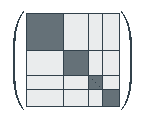
\includegraphics[height=0.8\linewidth]{../repos/hbp-paper/doc/aistats_talk/logo/hbp_logo}
    \href{https://github.com/f-dangel/hbp}{\texttt{github.com/f-dangel/hbp}}
  \end{center}} %
presents Hessian backpropagation (HBP), an extension of gradient backpropagation
to compute layer-wise curvature in sequential feedforward neural networks. Just
like gradient backpropagation recovers the gradient vectors in blocks that
correspond to layers, local curvature, \ie second-order partial derivatives of
the loss \wrt parameters in a layer can be evaluated by backpropagating
Hessians. Its computation is disentangled to the modular level, which allows for
an elegant and extensible implementation in analogy to gradient backpropagation.
We describe the backpropagation operations at the per-layer level, resulting in
an algorithm that computes local curvature in an automated fashion, and at the
same time as the gradient. Adaptations of the exact procedure recover positive
semi-definite block diagonal approximations (BDAs)---\eg of the GGN---and
recently proposed Kronecker-factored curvature approximations
\cite{martens2015optimizing,botev2017practical,wei2018bdapch} of the Hessian,
unifying their computation.

\begin{disclaimer}
  \Cref{chap:hbp} is based on the peer-reviewed conference
  paper with the following co-author contributions:

  \fullcite{dangel2020modular} \cite{dangel2020modular}

  \vspace{-1.75ex}

  \begin{center}
    \begin{tabular}[!h]{lrrrr}
      & \textbf{Ideas} & \textbf{Experiments} & \textbf{Analysis} & \textbf{Writing}
      \\
      \textbf{F.\,Dangel} & 70\,\% & 80\,\% & 70\,\% & 65\,\%
      \\
      S.\,Harmeling & 10\,\%& 10\,\% & 10\,\% & 10\,\%
      \\
      P.\,Hennig & 20\,\% & 10\,\% & 20\,\% & 25\,\%
    \end{tabular}
  \end{center}
\end{disclaimer}

\Cref{chap:backpack} \marginnote{%
  \Cref{chap:backpack}:
  \backpack: an efficient framework built on top of \PyTorch that extends the
  backpropagation algorithm.
  \begin{center}
    \vspace{-2ex} 
\includegraphics[height =
    0.8\linewidth]{../repos/backpack-paper/tex/logo/backpack_logo_github}
    \href{https://github.com/f-dangel/backpack}{\texttt{github.com/f-dangel/backpack}}
  \end{center}} %
further generalizes this idea and presents \backpack, an efficient framework
that extends the gradient backpropagation of \pytorch. The library provides
access to higher-order statistical information about the gradient distribution,
like individual gradients or an estimate of their variance, and structured
curvature information, like the Hessian/\ggn diagonal and block-diagonal
Kronecker-factored curvature approximations. This is achieved with slightly more
flexible implementations of AD functionality and by backpropagating additional
information through the graph. Importantly, most quantities add small overhead
to the gradient, making their exploration for research more attractive.

\begin{disclaimer}
  \Cref{chap:backpack} is based on the peer-reviewed
  conference publication with the following co-author contributions:

  \fullcite{dangel2020backpack} \cite{dangel2020backpack}

  \vspace{-1.75ex}

  \begin{center}
    \begin{tabular}[!h]{lrrrr}
      & \textbf{Ideas} & \textbf{Experiments} & \textbf{Analysis} & \textbf{Writing}
      \\
      \textbf{F.\,Dangel} & 33\,\% & 55\,\% & 45\,\% & 35\,\%
      \\
      F.\,Kunstner & 33\,\%& 45\,\% & 45\,\% & 45\,\%
      \\
      P.\,Hennig & 33\,\% & 0\,\% & 10\,\% & 20\,\%
    \end{tabular}
  \end{center}
\end{disclaimer}

\Cref{chap:cockpit}\marginnote{%
  \Cref{chap:cockpit}: \cockpit: a debugging tool
  for the training of deep neural networks.
  \begin{center}
    \vspace{-5ex} 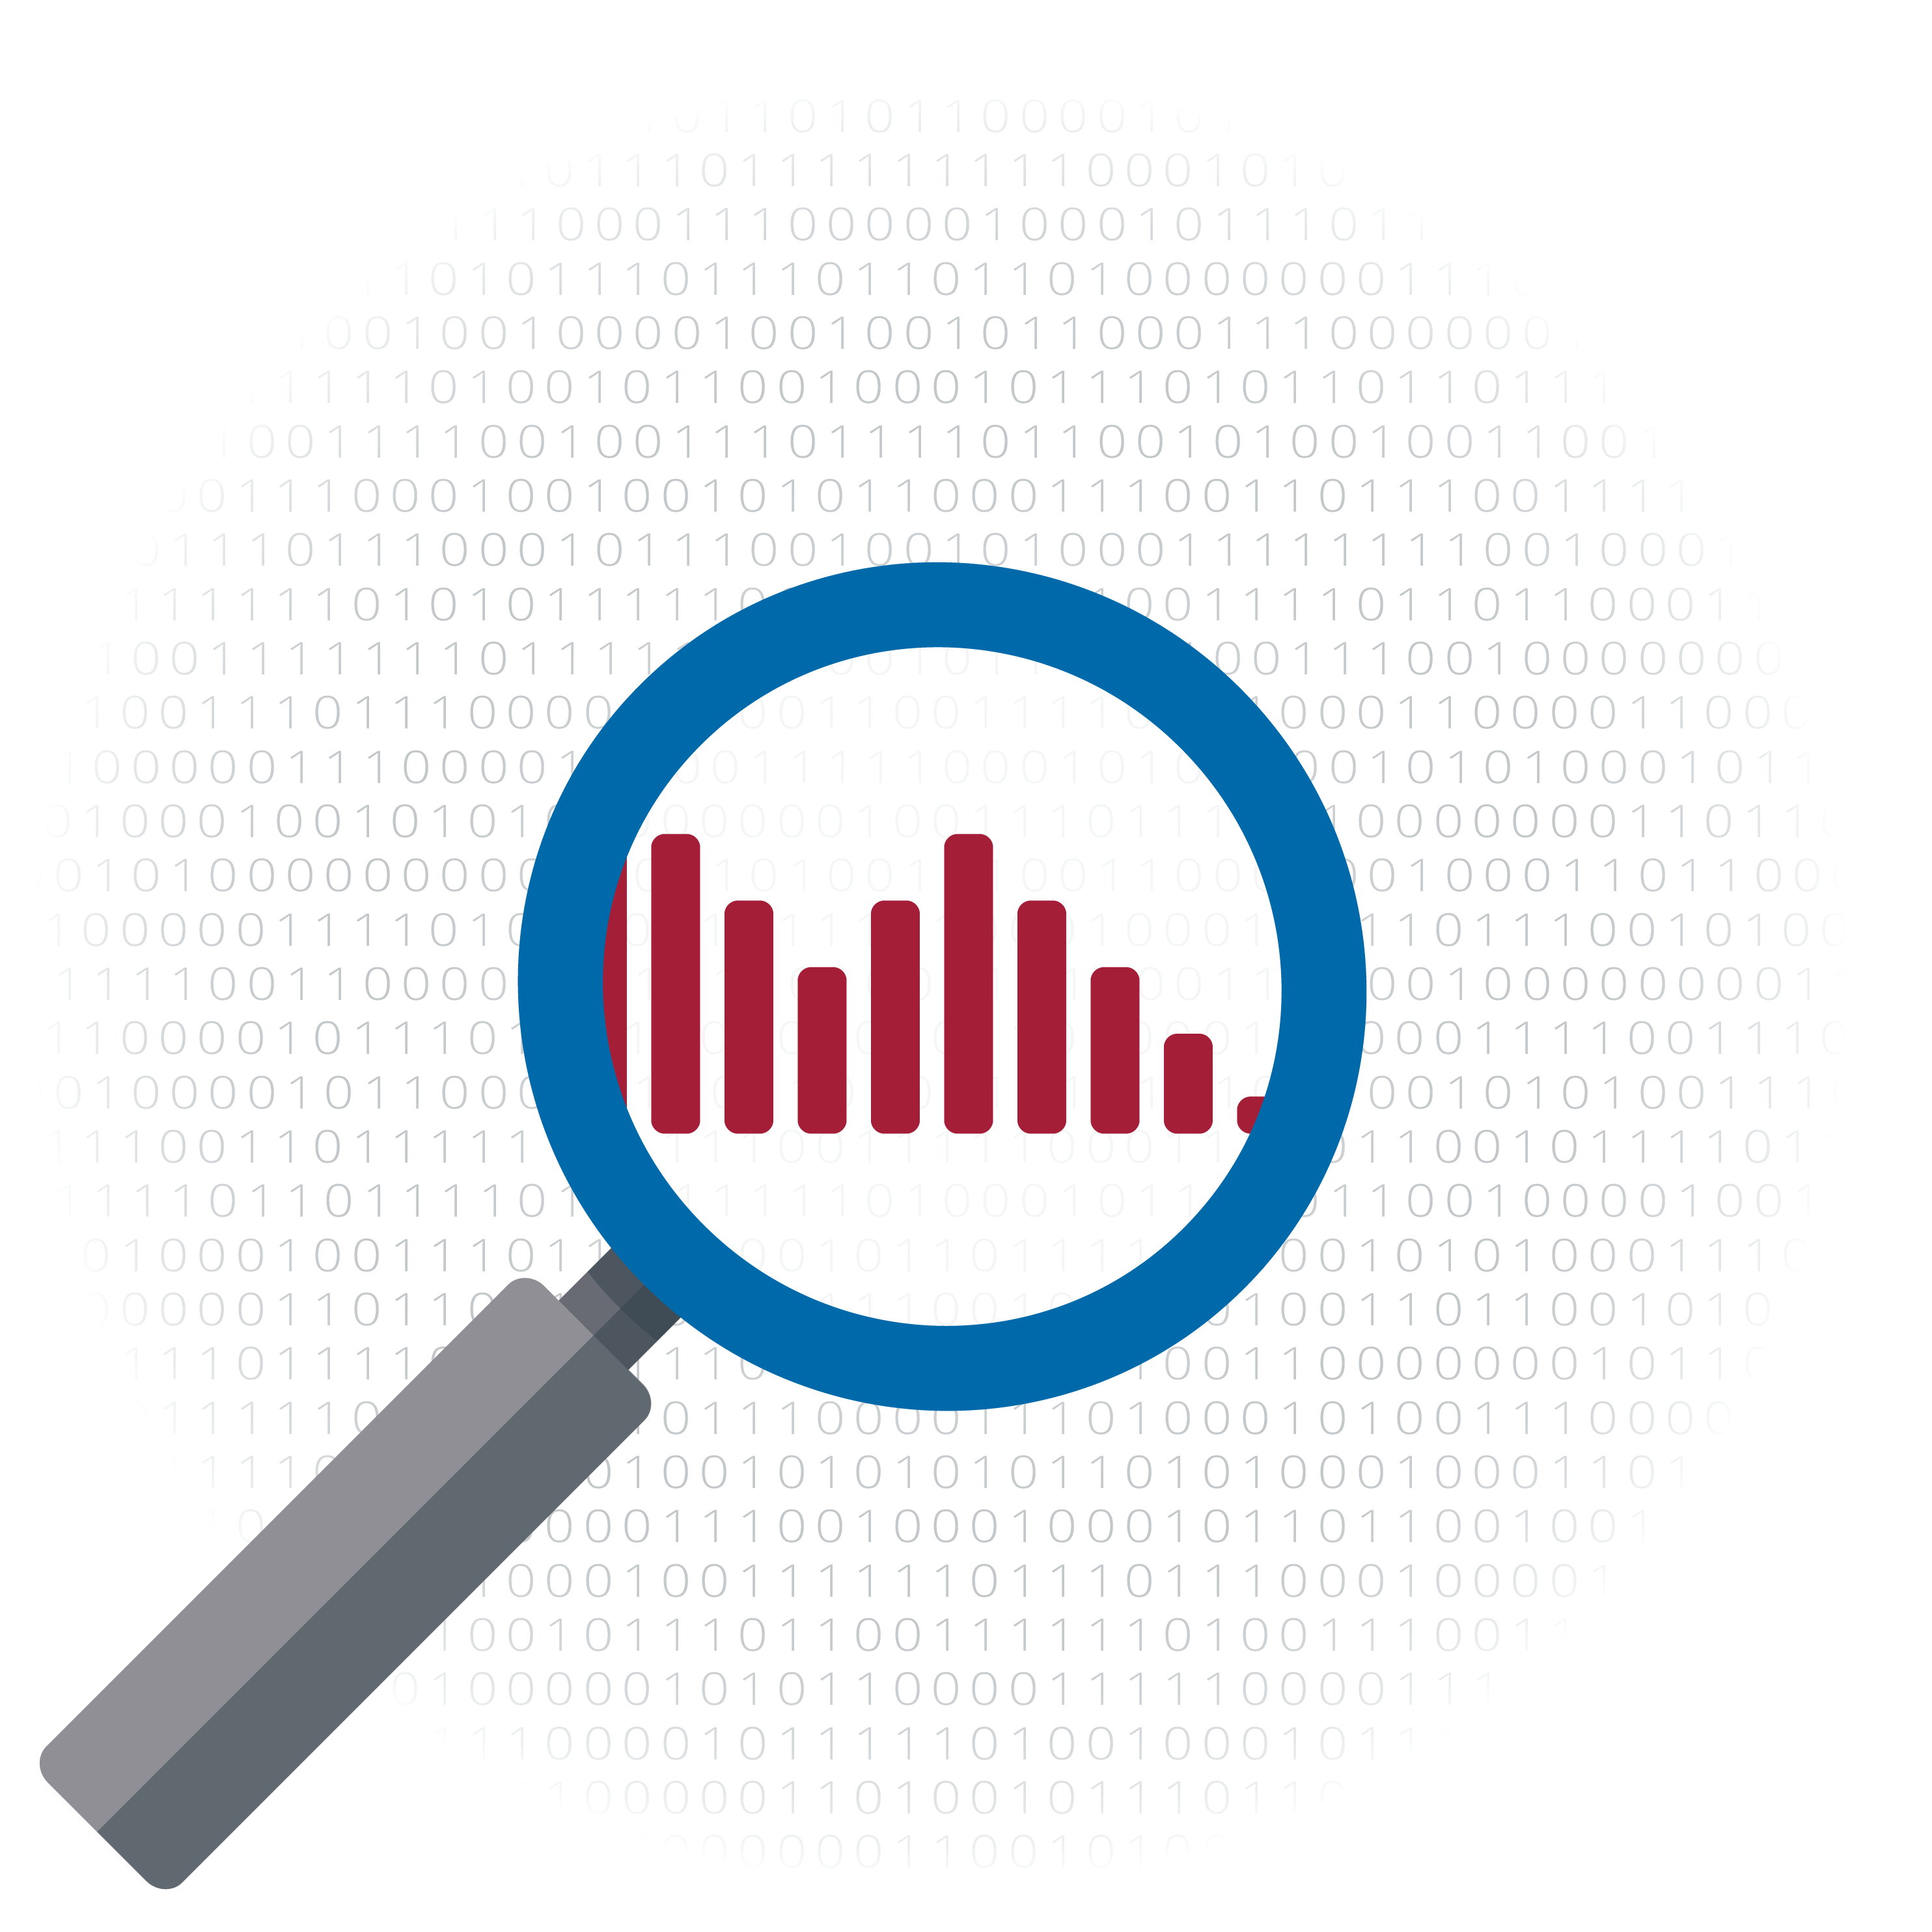
\includegraphics[height =
    0.8\linewidth]{../repos/cockpit/docs/source/_static/LogoSquare}
    \href{https://github.com/f-dangel/cockpit}{\texttt{github.com/f-dangel/cockpit}}
  \end{center}} %
introduces \cockpit, a live-monitoring debugging tool that consists of various
instruments which leverage higher-order information, efficiently provided by
\backpack. By providing a deeper look into the inner workings of neural networks
through the lens of this information, \cockpit can help identify bugs in the ML
pipeline, while keeping the computational overhead acceptable. This demonstrates
the utility of higher-order information to assist deep learning practitioners
and researchers to better understand their problems and conduct research.

\begin{disclaimer}
  \Cref{chap:cockpit} is based on the peer-reviewed
  conference paper with the following co-author contributions:

  \fullcite{schneider2021cockpit} \cite{schneider2021cockpit}

  \vspace{-1.75ex}

  \begin{center}
    \begin{tabular}[!h]{lrrrr}
      & \textbf{Ideas} & \textbf{Experiments} & \textbf{Analysis} & \textbf{Writing}
      \\
      F.\,Schneider & 45\,\%& 40\,\% & 40\,\% & 45\,\%
      \\
      \textbf{F.\,Dangel} & 40\,\% & 50\,\% & 40\,\% & 40\,\%
      \\
      P.\,Hennig & 15\,\% & 10\,\% & 20\,\% & 15\,\%
    \end{tabular}
  \end{center}
\end{disclaimer}

\Cref{chap:vivit} \marginnote{%
  \Cref{chap:vivit}: \vivit: efficient computation with the \ggn's low-rank
  structure.
  \begin{center}
    \vspace{-4ex} 
\includegraphics[height =
    0.8\linewidth]{../repos/vivit/docs/rtd/assets/vivit_logo}
    \href{https://github.com/f-dangel/vivit}{\texttt{github.com/f-dangel/vivit}}
  \end{center}}%
presents \vivit, a method that leverages the low-rank structure in the \ggn to
efficiently extract eigenvalues, eigenvectors, per-sample first- and
second-order directional derivatives, and Newton steps. In contrast to other
popular curvature approximations, \vivit is capable of tracking off-diagonal
curvature blocks, offers principled approximations to trade off cost and
accuracy, and allows studying noise in the curvature. Under the hood, \vivit's
quantities are efficiently computed during backpropagation, building on
\backpack's advanced AD functionality. This demonstrates how such functionality
enables investigations of unexplored structure in higher-order information which
may be used to develop novel algorithms and better understand challenges to make
them work in practice, \eg noise.

\begin{disclaimer}
  \Cref{chap:vivit} is based on the peer-reviewed journal paper with the
  following co-author contributions:

  \fullcite{dangel2022vivit} \cite{dangel2022vivit}

  \vspace{-1.75ex}

  \begin{center}
    \begin{tabular}[!h]{lrrrr}
      & \textbf{Ideas} & \textbf{Experiments} & \textbf{Analysis} & \textbf{Writing}
      \\
      \textbf{F.\,Dangel} & 50\,\% & 40\,\% & 40\,\% & 40\,\%
      \\
      L.\,Tatzel & 35\,\%& 50\,\% & 40\,\% & 45\,\%
      \\
      P.\,Hennig & 15\,\% & 10\,\% & 20\,\% & 15\,\%
    \end{tabular}
  \end{center}
\end{disclaimer}

\Cref{part:conclusion} summarizes the findings of this manuscript \wrt the
inital questions from \Cpageref{enum:background::Questions}, as well as their
impact and relation to the latest developments in the field. Finally, the
manuscript identifies future research directions for the presented extended AD
eco-system around \pytorch, and more broadly for the development of future ML
libraries.

%%% Local Variables:
%%% mode: latex
%%% TeX-master: "../thesis"
%%% End:
